\chapter{Development of Discrete Element Method for Pebble Bed Solid Breeders}\label{ch:modeling-development}

In this chapter I will cover the background of the discrete element method (DEM), the physics governing interactions of the distinct grains in the numerical framework, and 

%%%%%%%%%%%%%%%%%%%%%%%%%%%%%%%%%%%%%%%%%%%%%%%%%%%%%%%%%%%%%%%%%%%%%%%%%%%%%%%%%%%%%%%%%%%%%%%%%%%%%%%%%%%%
%%%%%%%%%%%%%%%%%%%%%%%%%%%%%%%%%%%%%%%%%%%%%%%%%%%%%%%%%%%%%%%%%%%%%%%%%%%%%%%%%%%%%%%%%%%%%%%%%%%%%%%%%%%%
%
% new section
%
%%%%%%%%%%%%%%%%%%%%%%%%%%%%%%%%%%%%%%%%%%%%%%%%%%%%%%%%%%%%%%%%%%%%%%%%%%%%%%%%%%%%%%%%%%%%%%%%%%%%%%%%%%%%
%%%%%%%%%%%%%%%%%%%%%%%%%%%%%%%%%%%%%%%%%%%%%%%%%%%%%%%%%%%%%%%%%%%%%%%%%%%%%%%%%%%%%%%%%%%%%%%%%%%%%%%%%%%%
\section{Grain-scale Modeling} \label{sec:modeling-dem}

The observable, macroscopic behavior of particulate, or granular, systems is a complex function of myriad particle interactions. Historically, empirical relationships have been used to describe these systems as if a continuous media, \textit{e.g.} the correlations for heat transfer discussed in \cref{sec:granular-ht-correlations}. But with the advent of the discrete element method by Cundall and Strack and the acceleration of computing power, it became practical to investigate these particulate systems at the particle scale without continuum assumptions \cite{Cundall1979}. With DEM, we track all the particles in the system in a Lagrangian manner. In the ensemble, the kinematics of each particle is tracked and updated based on balances (or imbalances) of forces or energy acting upon the particle. In this section I will work through equations governing interaction of particles in the DEM framework, the methods of computation, and the code used for implementation.



%~~~~~~~~~~~~~~~~~~~~~~~~~~~~~~~~~~~~~~~~~~~~~~~~~~~~~~~~~~~~~~~~~~~~~~~~~~~~~~~~~~~~~~~~~~~~~~~~~~~~~~~~~~~
% new subsection
%~~~~~~~~~~~~~~~~~~~~~~~~~~~~~~~~~~~~~~~~~~~~~~~~~~~~~~~~~~~~~~~~~~~~~~~~~~~~~~~~~~~~~~~~~~~~~~~~~~~~~~~~~~~
\subsection{Particle Dynamics}\label{sec:particle-dynamics}

The grains in our system are allowed translational and rotational degrees of freedom. In a packed bed, we can restrict our attention to local forces between particles; neglecting, say, non-contact forces such as van der Waals or electrostatic forces. In the first construct of momentum and temperature consideration, the particles are treated as if in vacuum. However a derivation of fluid interaction forces will be given in \cref{sec:modeling-cfd-dem}.

Assuming we know the contact forces acting upon particle $i$, Newton's equations of motion are sufficient to describe the particle kinematics. For translation and rotational degrees of freedom, the equations are:,
\begin{subequations}
\label{eq:newtons-second}
\begin{align}
	m_i  \ddt{\vec{r}_i}   & = m_i\vec{g} + \vec{f}_i \label{eq:newton-translational} \\
	I_i\dt{\vec{\omega}_i} & = \vec{T}_i \label{eq:newton-rotational}
\end{align}
\end{subequations}
where $m_i$ is the particle mass, $\vec{r}_i$ its location in space, $\vec{g}$ is gravity, $I_i$ is the particle's moment of inertia, and $\vec{\omega}_i$ its angular velocity.

The net contact force, $\vec{f}_i$, represents the sum of the normal and tangential forces from the total number of contacts, $Z$, acting on this grain.
\begin{equation}
 	\vec{f}_i = \sum_{j=1}^{Z} \vec{f}_{n,ij} + \vec{f}_{t,ij}
 \end{equation} 
and the net torque, $\vec{T}_i$, is similarly,
\begin{equation}
	\vec{T}_i = -\frac{1}{2}\sum_{j=1}^{Z} \vec{r}_{ij} \times \vec{f}_{t,ij}
\end{equation}

When Cundall and Strack first proposed the discrete element method, they used a linear spring-dashpot structure which saw the normal and tangential forces written as,
\begin{subequations}
\label{eq:dem-forces}
\begin{align}
	\vec{f}_{n,ij} &= k_{n,ij} \delta_{n,ij}\vec{n}_{ij} - \gamma_{n,ij} \vec{u}_{n,ij} 	\label{eq:normal-force} \\
	\vec{f}_{t,ij} &= k_{t,ij} \delta_{t,ij}\vec{t}_{ij} - \gamma_{t,ij} \vec{u}_{t,ij} 	\label{eq:tangential-force}
\end{align}
\end{subequations}
where Cundall and Strack defined the stiffness coefficients $k$ as constants and local damping coefficients $\gamma$ were proportional to them, $\gamma \propto k$, to allow dissipation of energy and the system to reach an equilibrium. 

Relative normal and tangential velocities, respectively, are decomposed from particle velocities,
\begin{subequations}
\label{eq:dem-velocities}
\begin{align}
	\vec{u}_{n,ij} &= (-(\vec{u}_i-\vec{u}_j)\cdot\vec{n}_{ij})\vec{n}_{ij} \\
	\vec{u}_{t,ij} &= (-(\vec{u}_i-\vec{u}_j)\cdot\vec{t}_{ij})\vec{t}_{ij}
\end{align}
\end{subequations}
with the unit vector $\vec{n}_{ij}$ pointing from particle $j$ to $i$

Similarly to the approach of Hertz (see \cref{sec:hertz-theory}), the surfaces of the two particles are allowed to virtually pass through each other (no deformation) resulting in normal and tangential overlaps of,
\begin{subequations}
\label{eq:dem-overlaps}
\begin{align}
	\delta_{n,ij} &= (R_i + R_j) - (\vec{r}_i -\vec{r}_j)\cdot \vec{n}_{ij} \\
	\delta_{t,ij} &= \int_{t_{c,0}}^{t} \vec{u}_{t,ij}\,\mathrm{d}\tau 
\end{align}
\end{subequations}
where the fictive tangential overlap, $\delta_{t,ij}$, is truncated to so the tangential and normal forces obey Coulomb's Law, $\vec{f}_{t,ij} \le \mu_i \vec{f}_{n,ij}$ with $\mu$ as the coefficient of friction of the particle.

The result is a relatively simple approach of calculating interaction forces between particles with \Cref{eq:dem-forces} based on the kinematics of velocity and position of interacting particles from \Cref{eq:dem-velocities} and \Cref{eq:dem-overlaps}, respectively. As DEM evolved and drew attention of more researchers, more complex formulas governing the spring-dashpot coefficients of \Cref{eq:dem-forces} emerged. But the core approach remained the same and the models all fall into the same family of so-called `soft particle' models of DEM. A well-composed summary of the different DEM force models is given by Zhu\etal.\cite{Zhu2007}

The method used in this work fits into the computational skeleton of Cundall and Strack's method but with non-linear spring-dashpot coefficients defined by simplified Hertz-Mindlin-Deresiewicz model. In this model, normal-direction stiffness coefficient of \Cref{eq:normal-force} is based on the Hertzian contact law (derived explicitly in \cref{sec:hertz-theory}). The tangential-direction stiffness coefficient follows from Brilliantov \cite{Brilliantov1996, Zhu2007, Langston1995}. Together, the spring coefficients are,
\begin{subequations}
\begin{align}
	k_{n,ij} &= \frac{4}{3}E_{ij}^*\sqrt{R_{ij}^*\delta_{n,ij}} \\
	k_{t,ij} &= 8 G_{ij}^*\sqrt{R_{ij}^*\delta_{t,ij}}
\end{align}
\end{subequations}
where $E_{ij}^*$ is the pair Young's modulus, $G_{ij}^*$ is the pair bulk modulus, and $R_{ij}^*$ is the relative radius. The terms are defined as,
\begin{subequations}
\begin{align}
	\frac{1}{E^*} &= \frac{1-\nu_1^2}{E_1} + \frac{1-\nu_2^2}{E_2} \\
	\frac{1}{R^*} &= \frac{1}{R_1} + \frac{1}{R_2} \\
	\frac{1}{G^*_{ij}} &= \frac{2(2+\nu_i)}{E_i} + \frac{2(2+\nu_j)}{E_j}
\end{align}
\end{subequations}

Similar to Cundall \& Strack's formulation, damping coefficients, $\gamma$, are included to account for energy dissipated from the collision of two particles \cite{DiRenzo2004, Tsuji1992, Tsuji1993}. Whether the damping coefficient is local or global and the exact form of the coefficient is more important for loosely confined granular systems and dictates the way the system approaches an equilibrium state.\cite{Makse2004} For the case of our tightly packed pebble beds, it suffices to use the efficient form of Refs.\cite{Dippel1996, Makse2004, Brilliantov1996, Zhang2005, Zhu2007},
\begin{subequations}
\begin{align}
	\gamma_n &= \sqrt{5}\beta_\text{diss}\sqrt{m^*k_{n,ij}} \\
	\gamma_t &= \sqrt{\frac{10}{3}}\beta_\text{damp}\sqrt{k_{t,ij} m^*}
\end{align}
\end{subequations}
with $\beta_\text{damp}$ as the damping ratio, and the pair mass, $\frac{1}{m^*} = \frac{1}{m_i} + \frac{1}{m_j}$. For a stable system with $\beta_\text{damp} < 1$, the damping ratio is related to the coefficient of restitution, $e$, as
\begin{equation}
	\beta_\text{diss} = -\frac{\ln{e}}{\sqrt{\ln^2{e}+\pi^2}}
\end{equation}

Systems to be solved by DEM models are therefore well-defined after specifying the few material properties of $E$, $\nu$, $\rho$, and $R_p$ and the interaction properties of $\mu$ and $e$.

Having expressed the contact mechanics of the discrete element method, we now must integrate the kinematic equations of the particles to resolve their evolutions. The most common means of marching in time with DEM is the velocity-Verlet algorithm \cite{Kruggel-Emden2008}. In this algorithm, \Cref{eq:newtons-second} are integrated with half-steps in velocity, full steps in position, and then finally the full step in velocity. In practice, the two half-steps in velocity are often compressed into a single, full step. The computational time integration steps are given in explicit detail in \cref{sec:dem-stability}. Owing to the explicit nature of the velocity-Verlet algorithm, stability is a constant concern with DEM simulations. Stable, critical time steps and means of circumventing unreasonably small time steps will also be addressed in \cref{sec:dem-stability}.

A last note. Throughout this work, I required a fully quiesced bed to act as a starting point or demarcate a mechanically steady-state bed. To determine when this occurs, the total kinetic energy of the entire ensemble is monitored and a packed bed is considered to have completely settled once the kinetic energy of the system is less than $10^{-8}$. A similar process was independently determined in a similar matter in the work of Ref.~\cite{Silbert2002}. 



%~~~~~~~~~~~~~~~~~~~~~~~~~~~~~~~~~~~~~~~~~~~~~~~~~~~~~~~~~~~~~~~~~~~~~~~~~~~~~~~~~~~~~~~~~~~~~~~~~~~~~~~~~~~
% new subsection
%~~~~~~~~~~~~~~~~~~~~~~~~~~~~~~~~~~~~~~~~~~~~~~~~~~~~~~~~~~~~~~~~~~~~~~~~~~~~~~~~~~~~~~~~~~~~~~~~~~~~~~~~~~~
\subsection{Granular Heat Transfer}\label{sec:dem-heat-transfer}

In a way analogous to handling particle momentums with Newton's laws of motion, Lagrangian tracking of energy of each particle is obtained via the first law of thermodynamics. Each particle is treated as a single distinct object and thus internal temperature gradients are assumed negligible. The temperature of particle $i$ is governed by
\begin{equation}\label{eq:thermoFirstLaw}
	m_iC_i\ddt{T_i} = Q_{s,i} + Q_{i}
\end{equation}
where $m$ and $C$ are the mass and the specific heat of the solid, respectively. Heat generation inside the particle is input with $Q_{s}$ and the total heat transferred to/from particle $i$ via conduction to all, $Z$, neighboring particles, is
\begin{equation}
	Q_i = \sum_{j=1}^Z Q_{ij}
\end{equation}

Assuming the particles are spherical, smooth, elastic, in vacuum, and we neglect radiation transfer between them, for two particles at temperatures $T_i$ and $T_j$, we quantify the amount of energy transferred between them with a contact conductance, $H_c$:
\begin{equation}\label{eq:pebble-conduction-heat-transfer}
    Q_{ij} = H_{c}(T_i - T_j)
\end{equation}

Batchelor and O'Brien\cite{Batchelor1977} developed a formulation of similar form and then made the brilliant observation that the temperature fields in the near-region of contacting spheres are analogous to the velocity potential of an incompressible, irrotational fluid passing from from one reservoir to another through a circular hole in a planar wall separating the two reservoirs. With the analogy, they could make use of the fluid flow solution to write the total heat flux across the circle of contact as \Cref{eq:pebble-conduction-heat-transfer} with heat conductance 
\begin{equation}\label{eq:batchelor-pebble-conductance}
    H_c = 2k_sa
\end{equation}
where $k_s$ is the conductivity of the contacting solids and $a$ is the radius of contact. Because we have assumed smooth, elastic, spherical solids, with Hertz theory (see \cref{sec:hertz-theory}), contact radius can be found as a function of contact normal force, $F_n$,
\begin{equation}
    a =  \left(\frac{3}{4}\frac{R^*}{E^*}\right)^{1/3}F_n^{1/3} 
\end{equation}
where, as before, $\frac{1}{E^*} = \frac{1-\nu_1^2}{E_1} + \frac{1-\nu_2^2}{E_2}$ and $\frac{1}{R^*} = \frac{1}{R_1} + \frac{1}{R_2}$. 

In the development of \Cref{eq:batchelor-pebble-conductance}, Batchelor and O'Brien had assumed the two contacting spheres to be of equal conductivity, $k_s$. Cheng\etal\cite{Cheng19994199} proposed a slightly modified conductance which allows for contacting materials of different thermal conductivity. They give,
\begin{equation}\label{eq:cheng-modification-batchelor}
    H_c = 2k^*a = 2k^* \left(\frac{3}{4}\frac{R^*}{E^*}\right)^{1/3}F_n^{1/3}
\end{equation}
where $\frac{1}{k^*} = \frac{1}{k_i} + \frac{1}{k_j}$. As well as being a more general, flexible formulation, the models analyzed by Cheng\etal\cite{Cheng19994199} are in good agreement with experiments.

Batchelor and O'Brien developed \Cref{eq:batchelor-pebble-conductance} with the assumption of two contacting particles in vacuum but, once developed, showed\cite{Batchelor1977} that this form is still valid when immersed in a fluid providing that the thermal conductivity ratio, $\kappa = \frac{k_s}{k_f}$, of solid and fluid is well above unity. The condition is expressed as,
\begin{equation}\label{eq:conductance-validity-fluid}
    \frac{a}{R^*} \kappa \gg 1
\end{equation}
The term $\frac{a}{R^*}$, from \cref{sec:hertz-theory}, is necessarily less than 1 for Hertz theory to be applicable. Thus for fluid in vacuum, the condition is identically satisfied but we must consider inaccuracies if we introduce an interstitial fluid with low conductivity ratios; for lithium ceramics in helium, the ratio is approximately $\kappa \approx 10$.

We step back from contact of a single pair of particles and consider a particle in an ensemble with many contacts. We must again consider the validity of applying \Cref{eq:cheng-modification-batchelor} at each contact. Vargas and McCarthy\cite{Vargas2002a}, propose introducing a conduction Biot number to relate resistance of heat transfer internal to a particle with resistance between particles,
\begin{equation}
    \Bi_c = \frac{H_c}{k^* d_p} = 2\frac{a}{d_p}
\end{equation}

Then if $\Bi_c \ll 1$, the individual energy transferred between each point of contact can be decoupled. The Biot number criteria is already satisfied for Hertz theory to be valid; having assumed that $\frac{a}{d_p} \ll 1$. Therefore the total heat transferred out of a single particle with $Z$ contacts, due to contact conductance, is the summed contribution of individual contacts, 
\begin{equation}
    Q_i = \sum_j^Z Q_{ij}
\end{equation}

Conductive heat transfer to neighboring particles comes from inter-particle conductance formulas. The form of contact conductance we use, from \Cref{eq:cheng-modification-batchelor}, which is built upon the solution of Batchelor and O'Brien\cite{Batchelor1977}, has been implemented by others in a variety of DEM studies\cite{Vargas2001, Chaudhuri2006, Zhou2009,Cheng19994199}. However, it should noted that in many other fields, the researchers are interested in such things as the parallel conduction through a stagnant interstitial gas\cite{Bu2013} or the temporary conduction during impact of fluidized beds\cite{Zhu2008,Zhang2011,Wu2011,Li2000}. In such cases, the formula for conductance can be quite different but are not appropriate for the physics of our packed beds. 


\subsubsection{Thermal Expansion}
The stresses predicted to act upon the solid breeder volume during operation of the fusion reactor arise from the differential rate of thermal expansion from the highly heated ceramic volume and the relatively cool structural container. Moreover, thermal settling motion is observed in pebble beds with cyclic heating \cite{Tanigawa:2010cr, Vargas2007, Chen2009, Divoux2008}. Both of those phenomena originate from effects of thermal expansion of individual particles in the ensemble. Therefore, I introduce a simple thermal expansion method into the DEM structure that updates the diameter of each particle as,
\begin{equation}
	d_{p,i} = d_{p_0,i}\left[1+\beta_i\left(T_i - T_0\right)\right]
\end{equation}
where $\beta_i$ is the thermal expansion coefficient (in units of \SI{1}{\per\kelvin}), $T_i$ is the temperature of the pebble at the current step, and $d_{0,i}$ is the initial diameter of the pebble at temperature $T_0$. The update of pebble diameter based on thermal expansion could be computed at every time step as it is not computationally expensive. All the same, I have left flexibility in the code to allow the computation at an arbitrary interval of time, typically every $\frac{N}{\Delta t} = \frac{10^4}{10^{-7}}$ in most models of ceramic pebble beds).



%~~~~~~~~~~~~~~~~~~~~~~~~~~~~~~~~~~~~~~~~~~~~~~~~~~~~~~~~~~~~~~~~~~~~~~~~~~~~~~~~~~~~~~~~~~~~~~~~~~~~~~~~~~~
% new subsection
%~~~~~~~~~~~~~~~~~~~~~~~~~~~~~~~~~~~~~~~~~~~~~~~~~~~~~~~~~~~~~~~~~~~~~~~~~~~~~~~~~~~~~~~~~~~~~~~~~~~~~~~~~~~
\subsection{Numerical Implementation of DEM}\label{sec:dem-solver}

The primary computational tool used in this study is LAMMPS (Large-scale Atomic/Molecular Massively Parallel Simulator) \cite{Plimpton1995}, a classical molecular dynamics code. The package of code, maintained by Sandia National Labs (http://lammps.sandia.gov), has many features making it particularly attractive for our use of granular material simulations. LAMMPS is open-source and written in highly-portable C++ allowing customization of any core modeling feature. LAMMPS runs with distributed-memory message-passing parallelism (MPI) and provides simple control (manual or automatic) of the spatial-decomposition of simulation domains for parallelizing. Perhaps most importantly, LAMMPS provides an efficient method for detecting and calculating pair-wise interaction forces; the largest consumer of run-time in the DEM algorithm \cite{Plimpton1995}. We build the LAMMPS core as a library to allow coupling LAMMPS features to other numerical tools. I use the scripting language of Python (Python 2.7) to write parent routines that pass information between LAMMPS objects while accessing all of Python's numeric and scientific libraries (\textit{e.g.} NumPy and SciPy). 

LAMMPS by default provides a rudimentary method of modeling of granular particles (the term `granular' in LAMMPS vernacular simply differentiates the discrete element of molecules or atoms from larger-scale granular particles of powders or pebbles); LAMMPS has been used for studying granular material since at least 2001 when Silbert\etal~studied granular flow on inclined planes \cite{Silbert2001}. However, the usefulness of LAMMPS for studying granular systems was greatly enhanced by LIGGGHTS (LAMMPS Improved for General Granular and Granular Heat Transfer Simulations), a suite of modules included on top of LAMMPS. LIGGGHTS has many academic and industrial contributors from around the world, with the code maintained as open-source by DCS Computing, GmbH.

Briefly, some notable features that LIGGGHTS brings to the LAMMPS environment include: built-in Hertz/Hooke pair styles with shear history, mesh importing for handling wall geometry, moving meshes, stress analysis of imported meshes, a macroscopic cohesion model, a heat transfer model, and improved dynamic load balancing of particles on processors\cite{Kloss2011,Kloss2012}. Both LIGGGHTS and LAMMPS are distributed under the open-source codes under terms of the Gnu General Public License.\cite{FreeSoftwareFoundationInc.2007}




%%%%%%%%%%%%%%%%%%%%%%%%%%%%%%%%%%%%%%%%%%%%%%%%%%%%%%%%%%%%%%%%%%%%%%%%%%%%%%%%%%%%%%%%%%%%%%%%%%%%%%%%%%%%
%%%%%%%%%%%%%%%%%%%%%%%%%%%%%%%%%%%%%%%%%%%%%%%%%%%%%%%%%%%%%%%%%%%%%%%%%%%%%%%%%%%%%%%%%%%%%%%%%%%%%%%%%%%%
%
% new section
%
%%%%%%%%%%%%%%%%%%%%%%%%%%%%%%%%%%%%%%%%%%%%%%%%%%%%%%%%%%%%%%%%%%%%%%%%%%%%%%%%%%%%%%%%%%%%%%%%%%%%%%%%%%%%
%%%%%%%%%%%%%%%%%%%%%%%%%%%%%%%%%%%%%%%%%%%%%%%%%%%%%%%%%%%%%%%%%%%%%%%%%%%%%%%%%%%%%%%%%%%%%%%%%%%%%%%%%%%%
\section{Young's Modulus Implementation in DEM for Ceramic Pebbles}\label{sec:exp-reduction-factor}

In all past DEM efforts for ceramic breeders, the validity of Hertz theory (see \cref{sec:hertz-theory} and \cref{sec:modeling-dem}) for describing the inter-particle contact force as a function of fictitious overlap is assumed. In our experimental test stand for crushing individual pebbles, our equipment was able to record accurate measurements of the force-travel relationship for each pebble, providing us with an opportunity to study the validity of the Hertzian contact laws. 

The derivation of the Hertz force can be found on page~\pageref{eq:hertz-normal-force} but the result is given again here for reference:
\begin{equation*}
  F_{n,ij} = \frac{4}{3}E_{ij}^* \sqrt{R_{ij}^*} \, \delta_{n,ij}^{3/2}
\end{equation*}
and, again, the pair Young's modulus and radius are
\begin{align*}
\frac{1}{E^*} & = \frac{1-\nu_i^2}{E_i} + \frac{1-\nu_j^2}{E_j} \\
\frac{1}{R^*} & = \frac{1}{R_i} + \frac{1}{R_j}
\end{align*}

In experiments where we press a ceramic pebble between two anvils, we measure the travel, $s$, rather than the pebble overlap, so we modify \Cref{eq:hertz-normal-force} to be represented in terms of travel ($s = 2\delta$). Furthermore, for a pebble ($R_i = R_p$) in contact with a smooth plane ($R_j \rightarrow \infty$), the relative radius is simply $R^* = R_p = d_p/2$. We write the Young's modulus of the pebble as $E_p$ and for the test stand's anvil as $E_s$; similarly for the Poisson ratios of the two materials. The Hertz force acting upon a pebble between anvils is then expressed as a function of the pebble and anvil properties as,
\begin{equation}\label{eq:contact-force}
        F = \left[\frac{1}{3}\frac{\sqrt{d_p}}{\frac{1-\nu_p^2}{E_p} + \frac{1-\nu_s^2}{E_s}}\right] s^{3/2}
\end{equation}


\begin{figure}[!t]
\centering
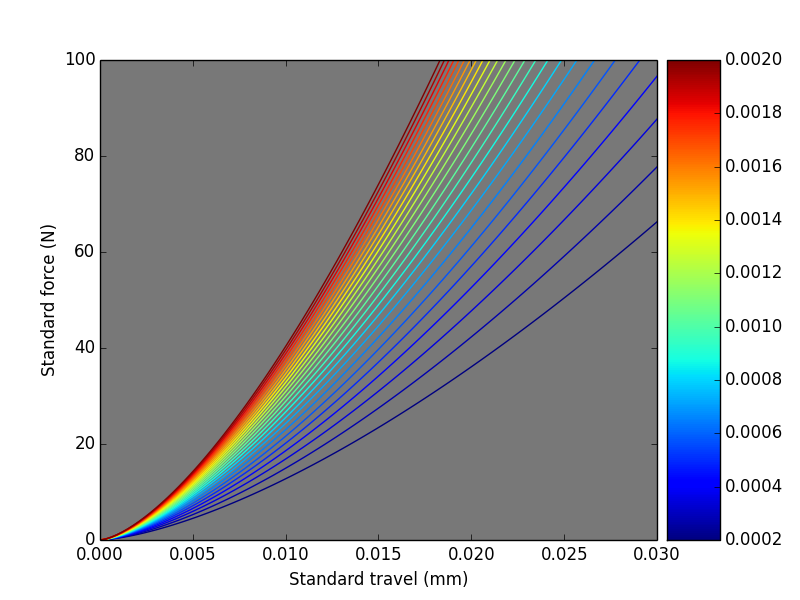
\includegraphics[width = \singleimagewidth]{figures/hertz-dp-dependence}
\caption{Hertzian responses of \lit~pebbles compressed between platens. The colormap shows pebble diameters in \si{m}. The diameters span an order of magnitude from $d_p = \si{0.2 mm}$ to $d_p = \si{2 mm}$.}\label{fig:hertz-dp-dependence}
\end{figure}


The Young's modulus and Poisson ratio of the test stand are known values that do not vary between pebble experiments. Similarly, in the application of Hertz theory, we also assume the Young's modulus and Poisson ratio of the ceramic are also known, constant values. In that case, for any given pebble diameter, the term inside $[\quad]$ ought to be composed entirely of constants for any given pebble; there would therefore be a single force-travel response possible -- based only on $s$. Using the material properties given in Ref.~\cite{Gierszewski1998} for \lit, we plot a set of parametric curves based on diameter over a range of travel. The properties we have used for the nickel-alloy anvil of our test stand and \lit~are given in Table~\ref{tab:hertz-dp-study-props}. The curves are given in Fig.~\ref{fig:hertz-dp-dependence}.

\begin {table}[htp] %
\caption{Material properties used for \lit~and nickel-alloy platen}
\label {tab:hertz-dp-study-props} \centering %
\begin {tabular}{ cccccc }
\toprule %
$E_\text{peb}$      &     $\nu_\text{peb}$  &   $E_\text{stand}$        &     $\nu_\text{stand}$    \\
(GPa)           &                   &   (GPa)               &                   \\\toprule
126             &   0.24                &   220                 &   0.27                \\\bottomrule
\end{tabular}
\end{table}

Figure~\ref{fig:hertz-dp-dependence} shows that, for a given pebble diameter, that is strictly obeying Hertz theory, there is only a single force-displacement curve it can follow. However, when experiments are performed on single pebbles of \lis~we see responses such as shown in the dashed lines of Fig.~\ref{fig:fzk-exp-colormap}. Similarly for the dashed lines of \lit~in Fig.~\ref{fig:nfri-exp-curves}. The diameters of the pebbles are mapped to the given colormap.

Contrary to the diameter dependence seen in Fig.~\ref{fig:hertz-dp-dependence}, the curves of Figs.~\ref{fig:fzk-exp-colormap}, and~\ref{fig:nfri-exp-curves} do not demonstrate a pure relationship between diameter and force. For comparison, the solid lines on the figures for each ceramic show the predicted Hertzian response as calculated by \Cref{eq:contact-force} based on the measured diameter of each pebble. For both the \lis~and \lit~pebbles, there are very few pebbles that show a measured force-travel response that is similar to the Hertzian prediction based on the material properties reported in literature. I conclude that variations in pebble diameter can not alone account for the variations in the force curves measured for the pebbles in our experiments. I hypothesize instead that variation in measured curves is due to each pebble having a Young's modulus that is reduced from the values measured from sintered blocks as reported in literature. Therefore each pebble displays a different apparent Young's modulus in the single pebble experiments. 

The apparent Young's modulus of each pebble is rooted in the manufacture which yields pebbles with slightly different internal structures. The differences in internal structure then cause the pebble to behave with different stiffnesses than the value expected from measurements of sintered pellets of lithium ceramics. In fact, the solid lines in Figs.~\ref{fig:fzk-exp-colormap}, and~\ref{fig:nfri-exp-curves}, as calculated from the measurements of sintered pellets, appear to be an upper limit to the pebbles. Therefore I consider pebbles will emerge with values less than the value from literature, $E_\text{lit}$ by some factor between 0 and 1. To quantify the deviation of each pebble's $E_\text{peb}$ from the sintered pellet, I introduce a $\kappa$ factor, which I define as the softening coefficient:

\begin{equation}
\kappa = \frac{E_\text{peb}}{E_\text{lit}}
\end{equation}
where
\[
\kappa \in [0,1]
\]

If each pebble has a unique $\kappa$ value, it would quantify the spread in elastic responses seen in the experiments. The values are found by assuming that the pebbles are, in fact, behaving in a Hertzian manner and I can fit a Hertzian curve to our experimental measurements. This permits backing-out a $\kappa$ value, or in other words the unique $E_\text{peb}$ of that pebble. The sintered pebble value of Young's modulus for \lis~is taken to be $E_\text{lit} = \si{90~GPa}$ and the value for \lit~to be $E_\text{lit}= \si{124~GPa}$. Then I iterate over all values of $\kappa\in[0,1]$ and compare the Hertzian response to that pebbles force-displacement curve. At each iteration, the L2-norm of the difference between Hertzian and experimental curves is used as the `error'. The L2 norm, $A$ for a given array, $a$ is 

\begin{equation}
||A||_F = \left[\sum_{i,j}\textrm{abs}(a_{i,j})^2\right]^{1/2}
\end{equation}

This is a convenient way to compare the error at every point along the force-displacement curves. When the error is minimized, the softening coefficient value corresponding to the minimum is recorded for that pebble. The Hertzian curves (in black) for the \lis~and \lit~pebbles are plotted in green against the experimental curves in Figs.~\ref{fig:fzk-exp-hertz}, and~\ref{fig:nfri-exp-hertz}, respectively. 

Many of the curves for \lis~in Fig.~\ref{fig:fzk-exp-hertz} seem to be fit well with a Hertzian curve using a modified Young's modulus. The value of Young's modulus found for each pebble is ordered and plotted in Fig.~\ref{fig:fzk-E-plot}; the Young's modulus of pebble numbers 0 to 4 are the very soft pebbles seen with very low forces over the range of travel seen in Fig.~\ref{fig:fzk-exp-hertz}. The majority of pebbles, however, behave with a Young's modulus between 30 and 70 \si{GPa}. On the upper end, a few pebbles acted very similar to their sintered pellet counterpart with approximate value of 90 \si{GPa}. 

The two batches of \lit~pebbles analyzed (Fig.~\ref{fig:nfri-exp-hertz}) are similarly fit well to pebbles with modified Hertzian curves. The apparent Young's modulii of the \lit~pebbles are given in Fig.~\ref{fig:nfri-E-plot}. These \lit~pebbles have a large distribution of stiffness, from between 20 to 120~GPa for the 1~mm pebbles and roughly 2 to 80~GPa for the 1.5~mm pebbles.


The $\kappa$ factor for this batch of \lis~pebbles is also given as a histogram in Fig.~\ref{fig:fzk-kappa-hist}. For the \lis~pebbles, the histogram resembles a normal distribution but for the large spike in pebbles with very small $\kappa$. The four softest pebbles mentioned previously display relatively flat responses to travel before reaching a point where there is a sharp increase in the $F-s$ slope. In the experiments, the flat sections of the curve occurred when the pebbles in the anvil were not perfectly spherical and rotated slightly under the application of a small load. Once the pebbles rotated into a flat spot that could take a normal load without any angular moment, the force increased quickly under further travel. In light of this, it is unreasonable to consider their $\kappa$ values as representing their true stiffness which was only measured near the end of the F-s compression trial. Neglecting the four outliers in the histogram of Fig.~\ref{fig:fzk-kappa-hist}, we are then left with a distribution much more closely resembling a normal probability distribution.

The histograms for the two batches of \lit~are given in Fig.~\ref{fig:nfri-kappa-hist}. The distributions for both batches of \lit~pebbles more closely resemble Snedecor's F distribution with many pebbles behaving with a very small $\kappa$, then a long tail of few pebbles with large $\kappa$.

In Figs.~\ref{fig:fzk-kappa-dp-scatter} and~\ref{fig:nfri-kappa-dp-scatter} we see scatter plots of the pebble diameters against $\kappa$ values for the different batches of lithium ceramic pebbles. A Pearson Correlation value was calculated for each of the batches to quantify a correlation between diameter and $\kappa$. For the \lis~pebbles, we find $R = 0.198$ which is a weak positive correlation. For the \lit~pebbles we have $R = -0.385$ for $\bar{d}_p = 1$~mm and $R = -0.201$ for $\bar{d}_p = 1.5$~mm. Both of these are weakly negatively correlated. 

The results of these single pebble experiments indicate that the Young's modulus traditionally used in DEM simulations for ceramic pebble beds in solid breeders is incorrect. Numerical recreations of the probability distribution curves will be used to apply $\kappa$ to pebbles in the ensemble. From the weak correlations between diameter and $\kappa$, we are free to ignore any diameter dependence when assigning $\kappa$ values in the DEM framework especially in light of the current implementation of monodisperse pebble beds. Therefore, numerically, when assigning Young's modulii to the particles in the ensemble, the $\kappa$ distribution will be applied in a random fashion.

\begin{figure}[!t]
\centering
    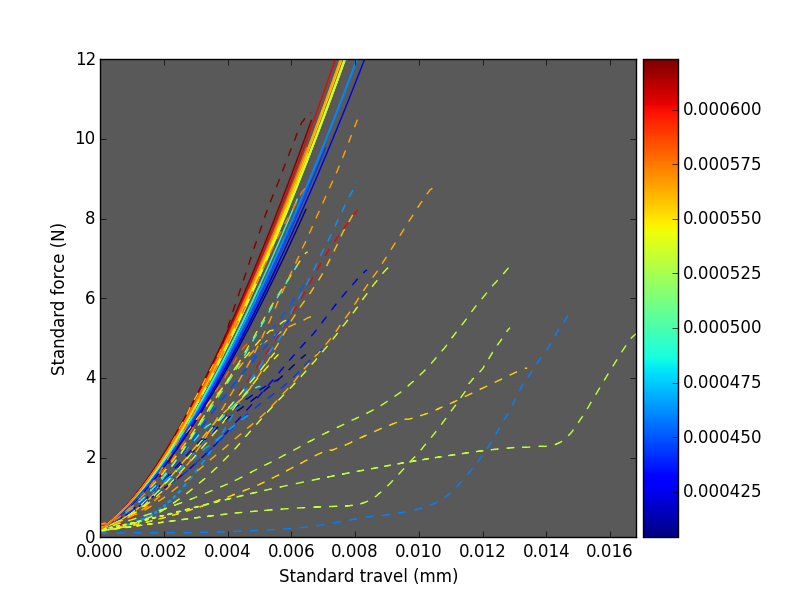
\includegraphics[width=\doubleimagewidth]{figures/fzk-data-w-ideal-hertz.png}
    \caption{Dashed lines are \lis~pebbles of approximately \si{0.5 mm} diameter. Solid lines are the Hertzian (Eq.\ref{eq:contact-force}) responses based on each pebble's measured diameter.}
    \label{fig:fzk-exp-colormap}
\end{figure}

\begin{figure}
        \centering
        \begin{subfigure}[b]{\doubleimagewidth}
                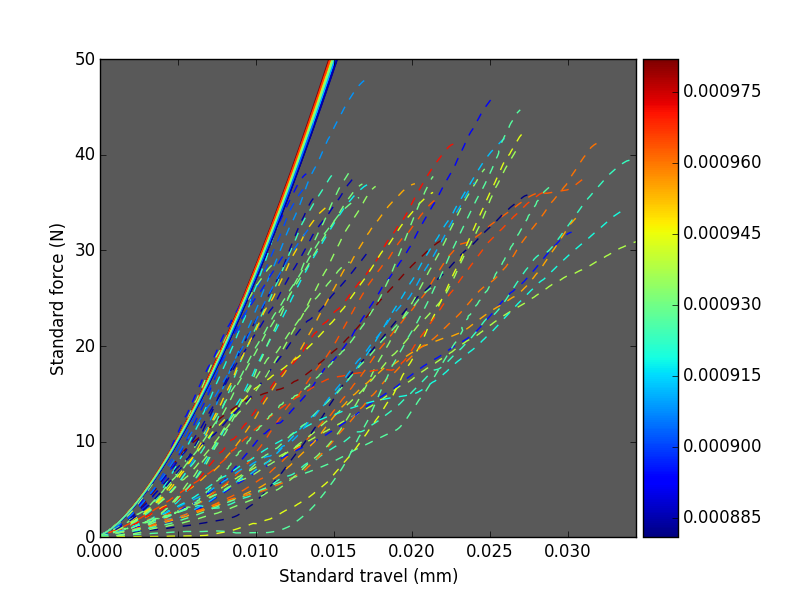
\includegraphics[width=\textwidth]{figures/nfri-1mm-data-w-ideal-hertz.png}
                \caption{$\bar{d}_p = 1$ mm}
                \label{fig:nfri-1-exp-colormap}
        \end{subfigure}
        ~
        \begin{subfigure}[b]{\doubleimagewidth}
                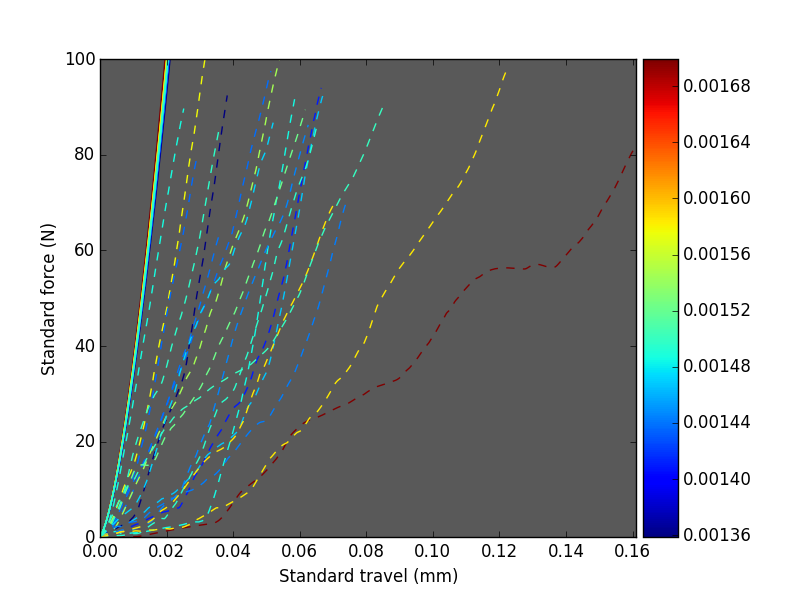
\includegraphics[width=\textwidth]{figures/nfri-1.5mm-data-w-ideal-hertz.png}
                \caption{$\bar{d}_p = 1.5$ mm}
                \label{fig:nfri-1.5-exp-colormap}
        \end{subfigure}
        \caption{Dashed lines are \lit~pebbles. Solid lines are the Hertzian (Eq.\ref{eq:contact-force}) responses based on each pebble's measured diameter.}\label{fig:nfri-exp-curves}
\end{figure}


\begin{figure}[!t]
\centering
    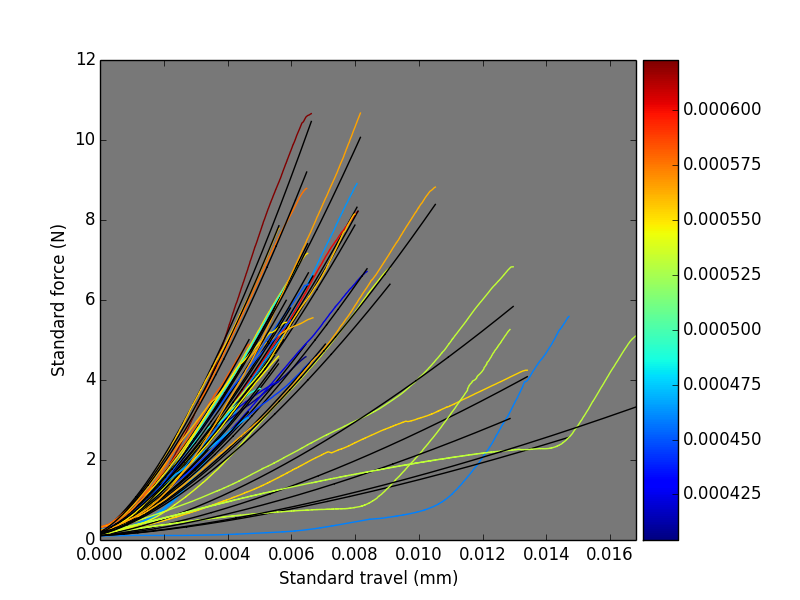
\includegraphics[width=\doubleimagewidth]{figures/fzk-hertz-colormap.png}
    \caption{Force-displacement curves for \lis~pebbles (in color) along with their Hertzian fits (in black) calculated with each pebble having a unique Young's modulus.}
    \label{fig:fzk-exp-hertz}
\end{figure}

\begin{figure}
        \centering
        \begin{subfigure}[b]{\doubleimagewidth}
                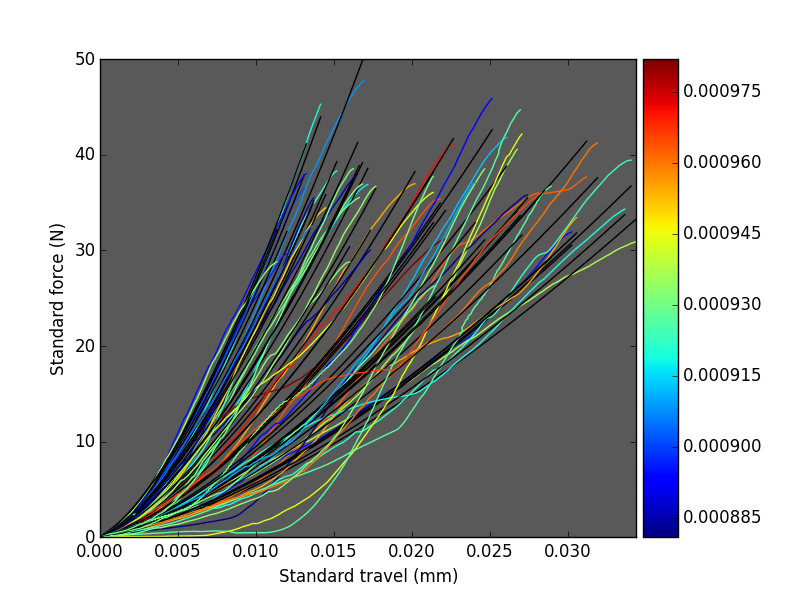
\includegraphics[width=\textwidth]{figures/nfri-1mm-hertz-colormap.png}
                \caption{$\bar{d}_p = 1$ mm}
                \label{fig:nfri-1-exp-hertz}
        \end{subfigure}
        ~
        \begin{subfigure}[b]{\doubleimagewidth}
                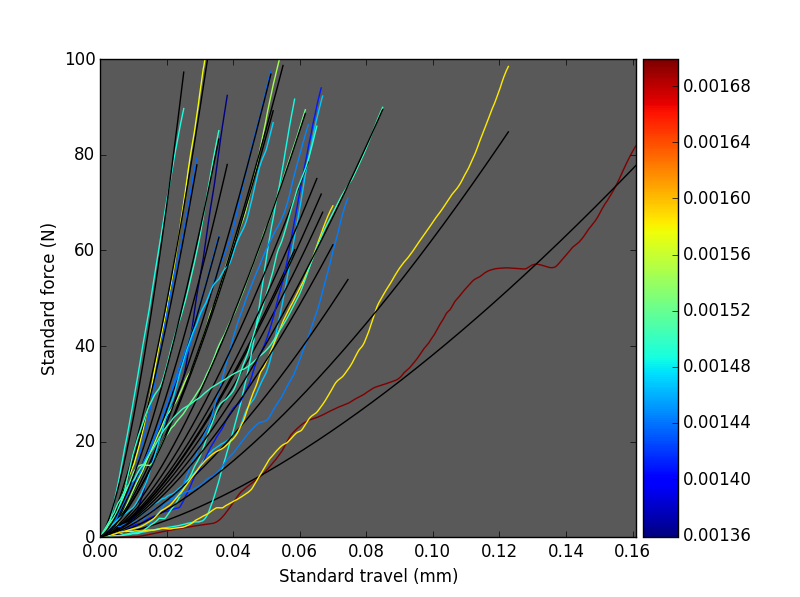
\includegraphics[width=\textwidth]{figures/nfri-1.5mm-hertz-colormap.png}
                \caption{$\bar{d}_p = 1.5$ mm}
                \label{fig:nfri-1.5-exp-hertz}
        \end{subfigure}
        \caption{Force-displacement curves for \lit~pebbles (in color) along with their Hertzian fits (in black) calculated with each pebble having a unique Young's modulus.}\label{fig:nfri-exp-hertz}
\end{figure}

\begin{figure}[!t]
\centering
    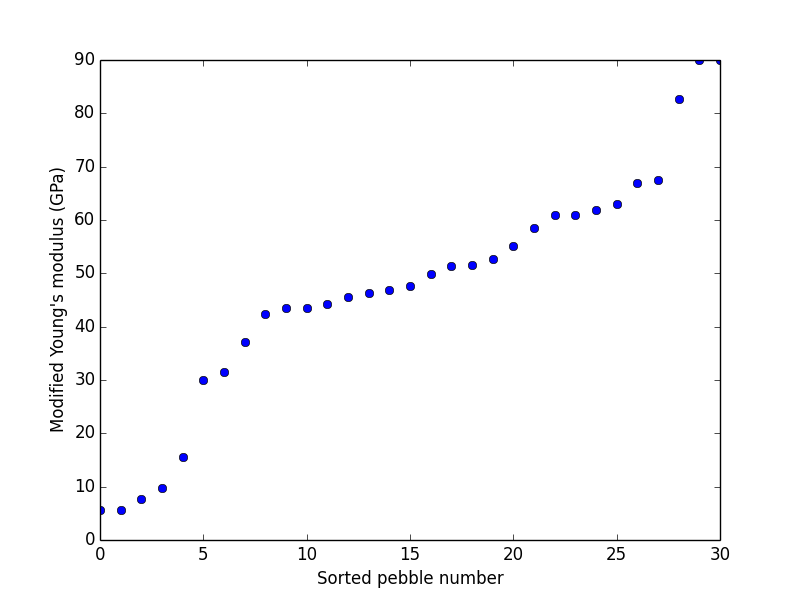
\includegraphics[width=\doubleimagewidth]{figures/fzk-E-plot.png}
    \caption{Distribution of modified Young's modulus for a batch of \lis~pebbles. Most pebbles responded to compression with a Young's modulus well below the sintered pellet value of \si{90 GPa}.}
    \label{fig:fzk-E-plot}
\end{figure}

\begin{figure}
        \centering
        \begin{subfigure}[b]{\doubleimagewidth}
                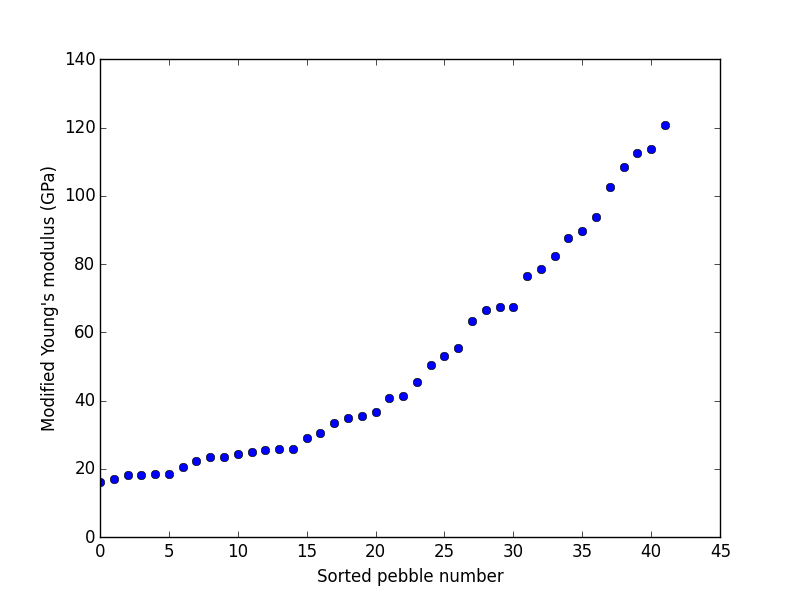
\includegraphics[width=\textwidth]{figures/nfri-1mm-E-plot.png}
                \caption{$\bar{d}_p = 1$ mm}
                \label{fig:nfri-1mm-E-plot}
        \end{subfigure}
        ~
        \begin{subfigure}[b]{\doubleimagewidth}
                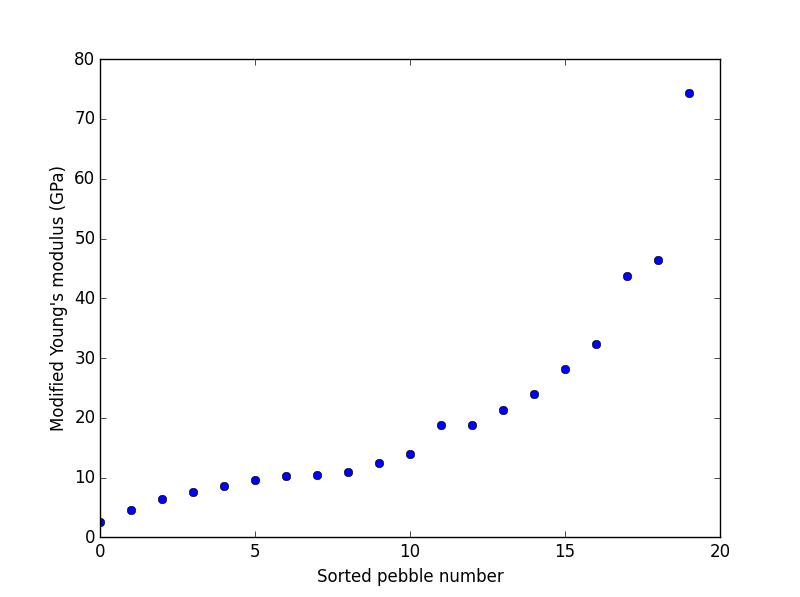
\includegraphics[width=\textwidth]{figures/nfri-1.5mm-E-plot.png}
                \caption{$\bar{d}_p = 1.5$ mm}
                \label{fig:nfri-1.5mm-E-plot}
        \end{subfigure}
        \caption{Distribution of modified Young's modulus for a batch of \lit~pebbles. All pebbles responded to compression with a Young's modulus well below the sintered pellet value of \si{126 GPa}.}\label{fig:nfri-E-plot}
\end{figure}


\begin{figure}[!t]
\centering
    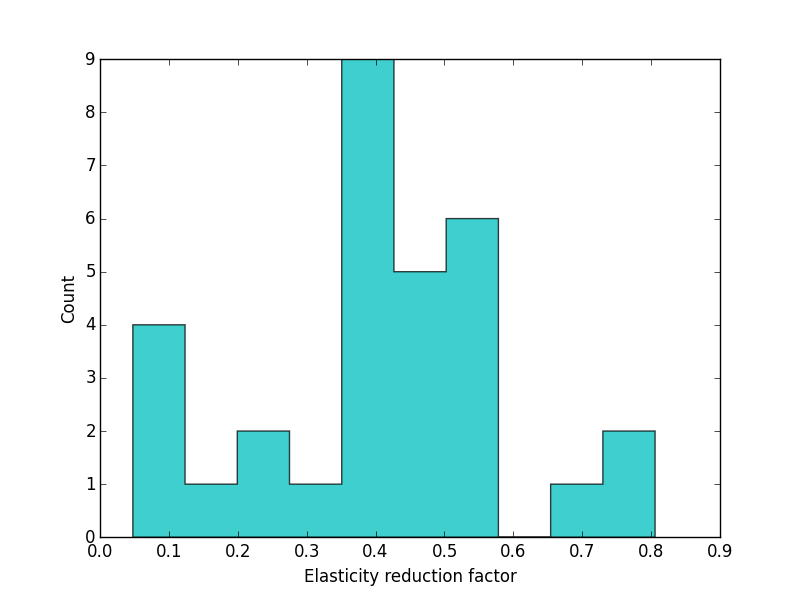
\includegraphics[width=\doubleimagewidth]{figures/fzk-kappa-histogram.png}
    \caption{Histogram of $\kappa$ for a batch of \lis~pebbles. Most pebbles responded to compression with a Young's modulus well below the sintered pellet value of \si{90 GPa}.}
    \label{fig:fzk-kappa-hist}
\end{figure}

\begin{figure}
        \centering
        \begin{subfigure}[b]{\doubleimagewidth}
                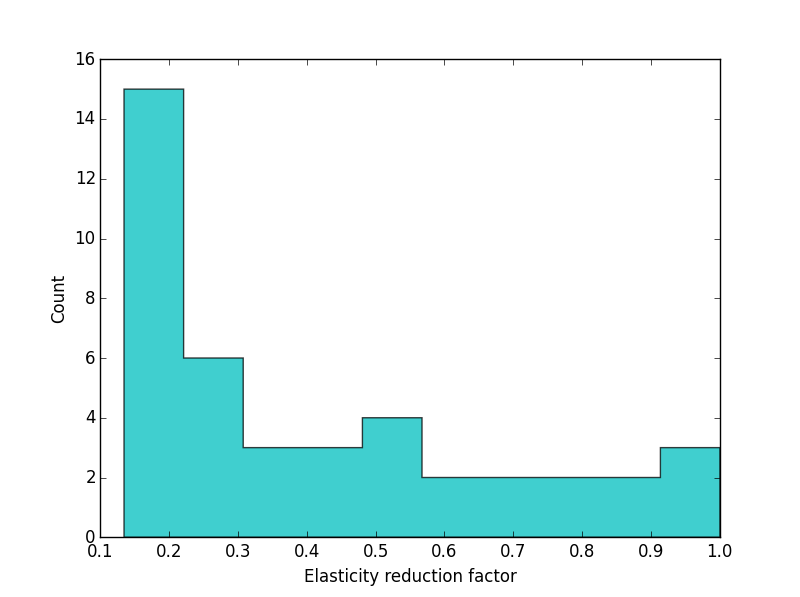
\includegraphics[width=\textwidth]{figures/nfri-1mm-kappa-histogram.png}
                \caption{$\bar{d}_p = 1$ mm}
                \label{fig:nfri-1mm-kappa-hist}
        \end{subfigure}
        ~
        \begin{subfigure}[b]{\doubleimagewidth}
                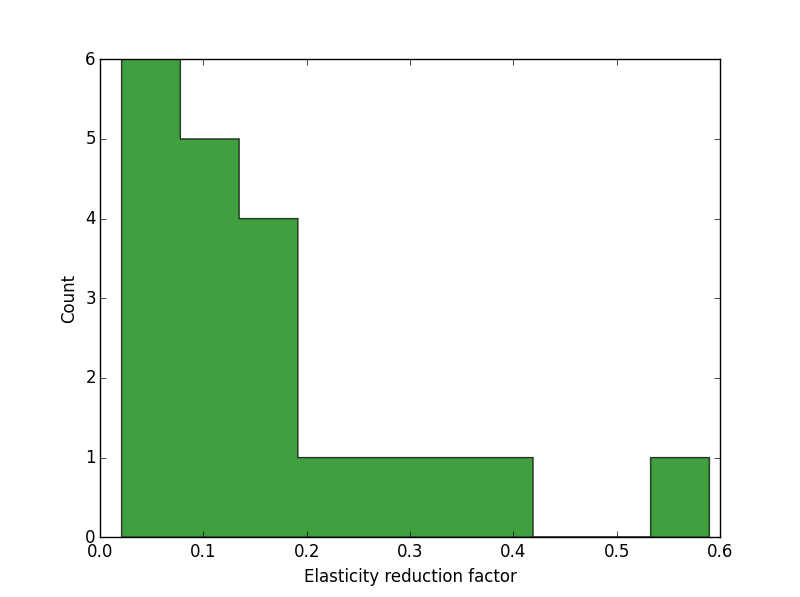
\includegraphics[width=\textwidth]{figures/nfri-1.5mm-kappa-histogram.png}
                \caption{$\bar{d}_p = 1.5$ mm}
                \label{fig:nfri-1.5mm-kappa-hist}
        \end{subfigure}
        \caption{Histogram of $\kappa$ for two batches of \lit~pebbles. All pebbles responded to compression with a Young's modulus well below the sintered pellet value of \si{126 GPa}.}\label{fig:nfri-kappa-hist}
\end{figure}


\begin{figure}[!ht]
\centering
    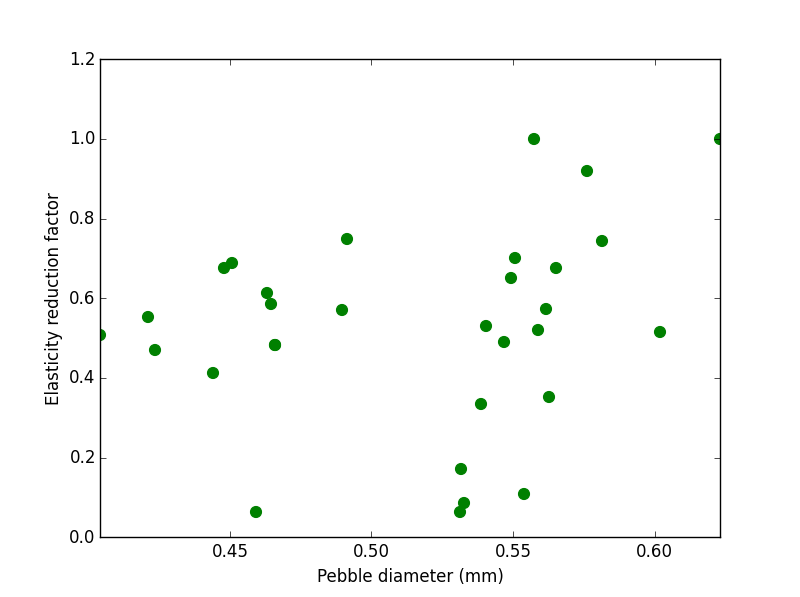
\includegraphics[width=\doubleimagewidth]{figures/fzk-kappa-dp-scatter.png}
    \caption{Scatter of $\kappa$ against pebble diameter for a batch of \lis~pebbles showing almost no relationship between apparent stiffness and diameter.}
    \label{fig:fzk-kappa-dp-scatter}
\end{figure}

\begin{figure}
        \centering
        \begin{subfigure}[b]{\doubleimagewidth}
                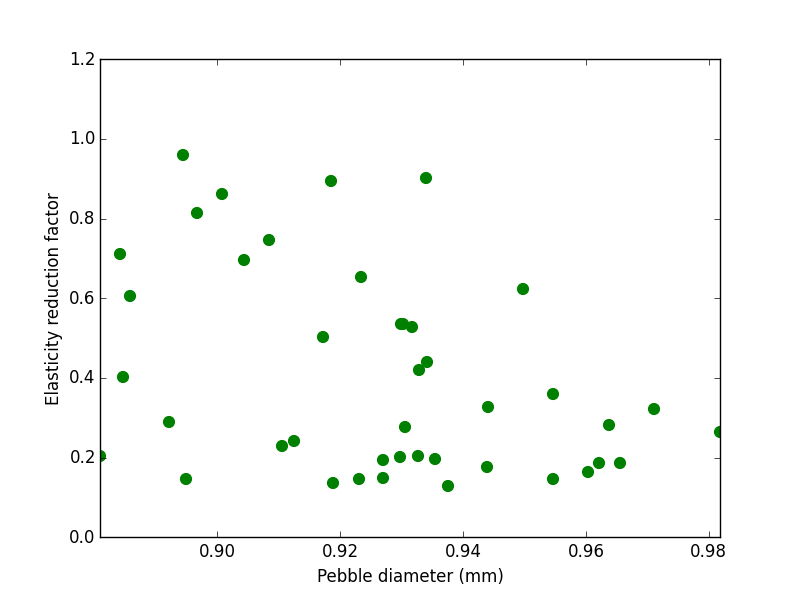
\includegraphics[width=\textwidth]{figures/nfri-1mm-kappa-dp-scatter.png}
                \caption{$\bar{d}_p = 1$ mm}
                \label{fig:nfri-1mm-kappa-dp-scatter}
        \end{subfigure}
        ~
        \begin{subfigure}[b]{\doubleimagewidth}
                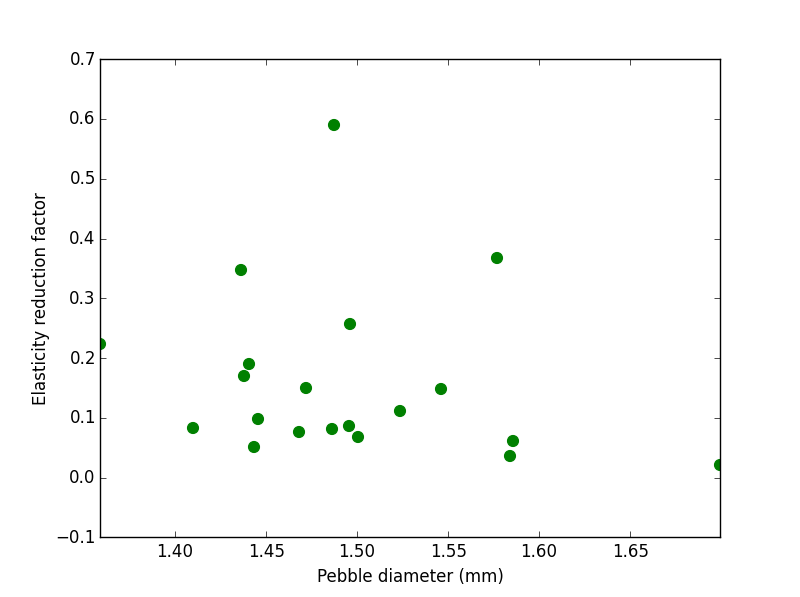
\includegraphics[width=\textwidth]{figures/nfri-1.5mm-kappa-dp-scatter.png}
                \caption{$\bar{d}_p = 1.5$ mm}
                \label{fig:nfri-1.5mm-kappa-dp-scatter}
        \end{subfigure}
        \caption{Scatter of $\kappa$ against pebble diameter for two batches of \lit~pebbles showing almost no relationship between apparent stiffness and diameter.}\label{fig:nfri-kappa-dp-scatter}
\end{figure}

\FloatBarrier


%~~~~~~~~~~~~~~~~~~~~~~~~~~~~~~~~~~~~~~~~~~~~~~~~~~~~~~~~~~~~~~~~~~~~~~~~~~~~~~~~~~~~~~~~~~~~~~~~~~~~~~~~~~~
% new subsection
%~~~~~~~~~~~~~~~~~~~~~~~~~~~~~~~~~~~~~~~~~~~~~~~~~~~~~~~~~~~~~~~~~~~~~~~~~~~~~~~~~~~~~~~~~~~~~~~~~~~~~~~~~~~
\subsection{Comparison of Young's Modulii Used in DEM Simulations}\label{sec:dem-studies-youngs-modulus}

The discrete element method is used by many ceramic breeder researchers to model the interaction of individual pebbles in an ensemble.\cite{An20071393, Lu2000, Zhao2010, Gan:2010uq, Annabattula2012a, VanLew2014} In the past studies, the Young's modulus of the ceramic materials used in DEM simulations was taken from historical data, for instance lithium metatitanate from Ref.~\cite{Gierszewski1998}. However, in the previous section I proposed a modification of the Young's modulus to be used in DEM simulations for a batch of ceramic pebbles based on the `softening' seen of most pebbles in experiments. The force-displacement curves of Figs~\ref{fig:fzk-exp-hertz} and~\ref{fig:nfri-exp-hertz} demonstrate how far from the ideal Hertzian curves the majority of of ceramic pebbles behave.

The Hertzian force is linearly proportional to the pair Young's modulus of contacting spheres. Based on the $\kappa$ values found in \cref{sec:exp-reduction-factor}, the apparent Young's modulii of \lis~and \lit~are, on average, less than half the values given for sintered materials in literature. For the case of \lit, the average value was closer to only 10\% of the value from literature. Thus the actual contact forces in pebble beds may be 10\% of the values found from DEM simulations with incorrect Young's modulus! The contact force is a critical value for determining the conduction heat transport between pebbles as well as damage prediction. It is crucial to use proper material properties in our simulations in order to have dependable predictions of pebble crushing events and heat transfer. In this section, I will compare a number of pebble beds under numerical simulations of uniaxial compression tests. One set of beds will be composed of pebbles with the single Young's modulus from literature and the other set will be composed of pebbles with a distribution of Young's modulii that fit the distribution from experiments.
%~~~~~~~~~~~~~~~~~~~~~~~~~~~~~~~~~~~~~~~~~~~~~~~~~~~~~~~~~~~~~~~


\subsubsection{Numerical Setup}
%In pebble bed breeder units, the stresses on the pebble regions are a result of thermal expansion of the relatively hot pebbles contained by relatively cool container walls. This process is a function of the coefficient of thermal expansion of the pebbles and their elevated temperature; the confined strain relates to a stress. 
The pebble beds are modeled as undergoing a standard uniaxial compression up to 6 MPa while measuring the macroscopic stress-strain for some parametrically varied pebble beds. At the moment of maximum stress, we can investigate the differences in contact forces of the different pebble beds.

Our pebble ensemble is composed of \SI{0.5}{\milli\meter} diameter \lis~pebbles. The pebble beds are initiated and packed in the same manner as \cref{sec:dem-studies-effective-conductivity} (more details can be found in that section). There are two main bed groups. Set A: three beds (A.1-3) containing a single type of pebble with $E$ = \si{90 GPa}. Set B: four beds (B.1-4) containing ten types of pebbles with their Young's modulus assigned in a discrete, random way to satisfy the distribution seen from experimental data. For the DEM study, I fit the \lis~pebbles with a Weibull distribution of shape parameter $\sigma = 1.6$ where the average stiffness was $\bar{E} = 49$~GPa. The description of the two sets of pebble beds is visually represented in Fig.~\ref{fig:dem-types}. The pebble bed geometry was also the same used in the study of Ref.~\cite{VanLew2014}~: two virtual walls in the x-direction located at $x_\text{lim} = \pm 20 R_p$, periodic boundaries at the limits of $y_\text{lim} = \pm 15 R_p$, and a total of 8000 pebbles packed into the volume to an approximate height of $z_\text{lim} = 20 R_p$.

Among both sets, a parametric study was done on pebble radius and coefficient of friction. The radii of pebbles in beds A.1, A.2, B.1, and B.2 were constant at $R_p$=.25 mm. The radii of pebbles in beds A.3, B.3, and B.4 followed a Gaussian distribution about $\bar{R}_p$ = 0.25 mm: $\mu_d = R_p$ and $\sigma_d = R_p$. The coefficient of friction was set at $\mu = 0.2$ for beds A.1, A.3, B.1, and B.3; the coefficient of friction was $\mu = 0.3$ for beds A.2, B.2, and B.4.


\begin{figure}[t]
  \centering
  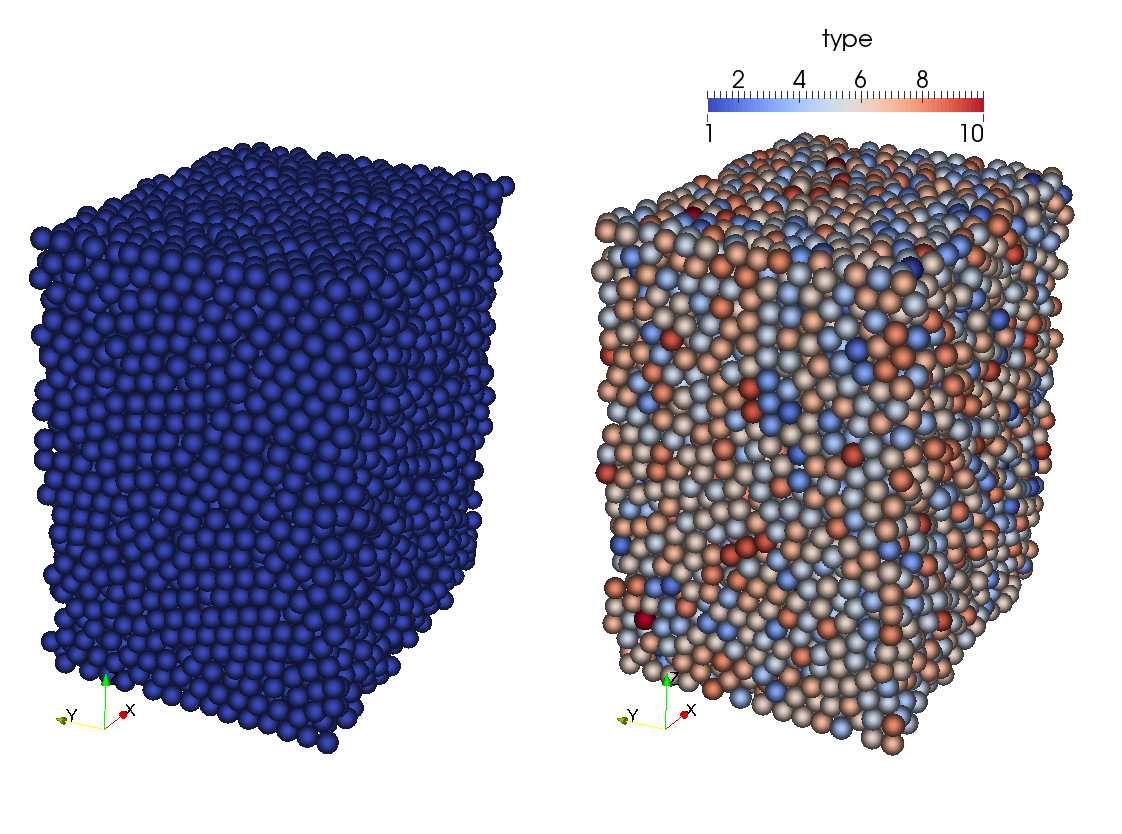
\includegraphics[width=\singleimagewidth]{figures/DEM-types}
  \caption{On the left, set A, a pebble bed with a single type, of $E = 120$ GPa. On the right, set B, is a pebble bed with 10, randomly distributed types; each type corresponds to a reduced, apparent Young's modulus as derived from experimental data.}\label{fig:dem-types}
\end{figure}



%~~~~~~~~~~~~~~~~~~~~~~~~~~~~~~~~~~~~~~~~~~~~~~~~~~~~~~~~~~~~~~~
\subsubsection{Results from Uniaxial Compression}


A constant-velocity, uniaxial compression was applied to the pebble beds. A single cycle up to \SI{6}{\mega\pascal} then down to \SI{0}{\mega\pascal} was used on all the beds. The macroscopic measurements of stress-strain are shown for all the pebble beds in Fig.~\ref{fig:stress-strain}.

\begin{figure}[t]
  \centering
  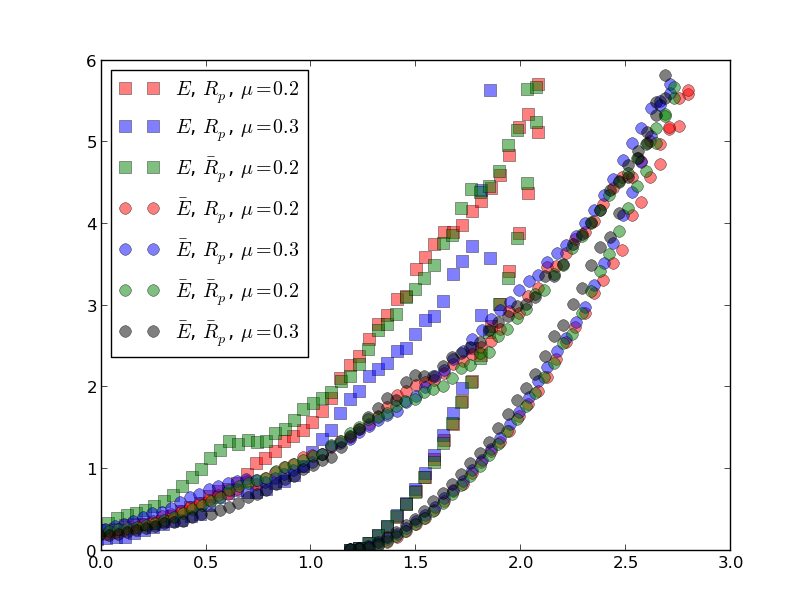
\includegraphics[width=\singleimagewidth]{figures/stress-strain}
  \caption{Stress-strain responses of pebble beds with: squares, constant Young's modulus; and circles, Gaussian distribution of Young's modulus. The constant Young's modulus beds all had much firmer responses for all parametric cases studied here.}\label{fig:stress-strain}
\end{figure}

Naturally, the pebble beds with smaller Young�s modulus (with circle markers) are more compliant to external loads. The result is true regardless of the coefficient of friction or distribution of pebble radius studied here. Group B moved to an average strain of about 2.6\% at \SI{6}{\mega\pascal}, by comparison the beds of Group A only had strained 1.9\% on average to reach the same stress. Among the beds of each group, pebble beds with constant radius pebbles behaved virtually the same as similar pebble beds with a Gaussian distribution on radius. An increase in the coefficient of friction had a moderate impact on the overall stress-strain response. 


The parametric study here shows that the largest contributor to stress-strain response is the Young�s modulus. The coefficient of friction and radius distribution had comparatively insignificant influence. A pebble bed geometry more directly comparable to oedometric compression experiments should be used to allow direct comparison and validation of the numerical models.


At the point of peak stress for each bed, I use DEM results to visualize the distribution of contact forces among all pebbles in the ensemble. A plot of the probability distributions of all the beds together, Fig.~\ref{fig:all-contact-forces}, shows that the majority of the contacts in all the beds are equally small. There are a few overall trends we observe from the results however. The pebble beds with the constant Young's modulus are always higher for their comparable version with distributed Young's modulus. For pebble beds with comparable Young's modulii and radii, higher coefficients of friction generally have higher peak contact forces. Pebble beds' radius distributions have much less impact on peak contact forces than either coefficient of friction or Young�s modulus. Another method of comparing overall contact force distributions is to consider predictions on pebble cracking which assigns a strength value at random to pebbles in the bed (details are given in \cref{sec:exp-reduction-factor}). At the point of maximum stress, this is done and the results are shown in Table~\ref{tab:num-crush-percent}.

While overall the predicted number of broken pebbles is small, we compare similar parameteric pebble beds and in each case pebble beds with modified Young�s modulus overall predict smaller percentages of broken pebbles. Pebble crushing is a major topic for the overall evaluation of the feasibility of ceramic pebble beds in fusion reactors. This study reveals that past DEM work on pebble crushing, such as Ref.~\cite{Annabattula2012a,Annabattula2014,Zhao2013}, were likely over-predicting the extent of crushing if the Young's modulus used in the study was much larger than the realistic response of individual pebbles.

\begin{figure}[t]
  \centering
  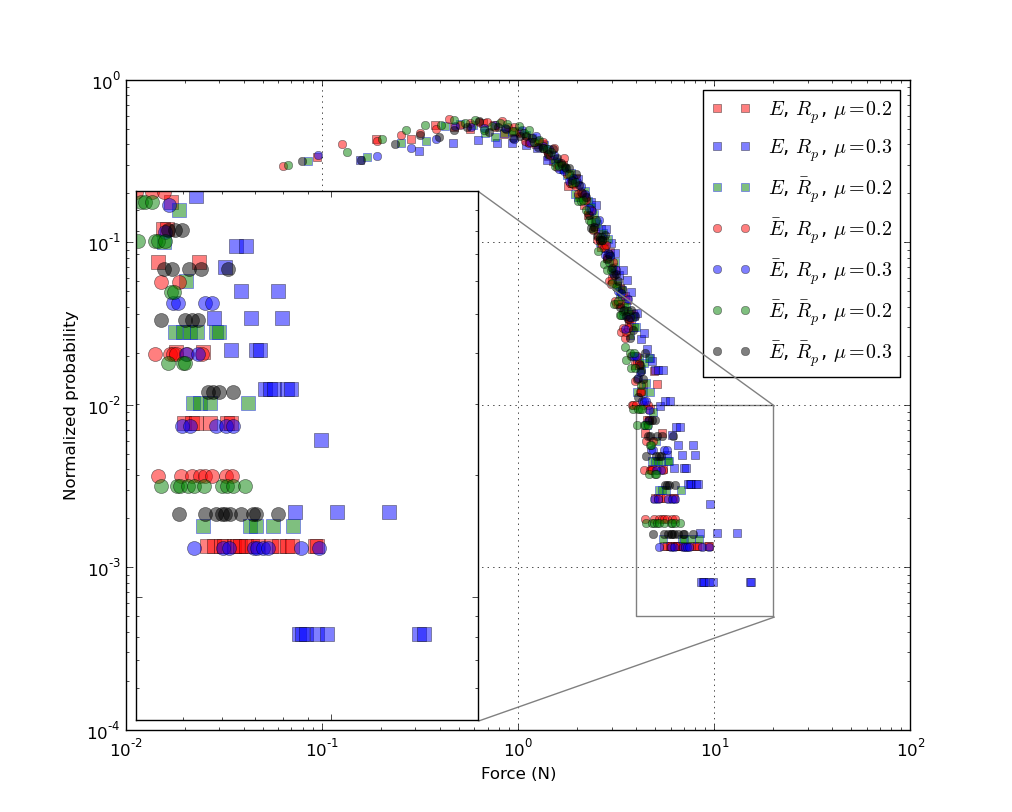
\includegraphics[width=\singleimagewidth]{figures/all-contact-forces}
  \caption{Probability distribution of contact forces in all the pebble beds studied here. Elastic moduli value is the largest contributor to higher peak contact forces among pebbles.}\label{fig:all-contact-forces}
\end{figure}


\begin{table}[t]
\caption{Comparisons for the two styles of Young's modulii used in the study. }
\label{tab:num-crush-percent}\centering
\begin{tabular}{llS[table-format=3.2]}
\toprule
Bed label		& 		Parameters 								&	\text{Predicted crushed}			\\
				& 												&	\multicolumn{1}{r}{\text{\%}}		\\\otoprule
A.1				& 		$E$, $R_p$, $\mu = 0.2$          		&	0.3									\\\midrule
A.2				& 		$E$, $R_p$, $\mu = 0.3$     			&	1.0									\\\midrule
A.3				& 		$E$, $\bar{R}_p$, $\mu = 0.2$			&	0.9									\\\midrule
B.1				& 		$\bar{E}$, $R_p$, $\mu = 0.2$			&	0.6									\\\midrule
B.2				& 		$\bar{E}$, $R_p$, $\mu = 0.3$			&	0.8									\\\midrule
B.3				& 		$\bar{E}$, $\bar{R}_p$, $\mu = 0.2$		&	0.4									\\\midrule
B.4				& 		$\bar{E}$, $\bar{R}_p$, $\mu = 0.3$		&	0.7									\\\bottomrule
\end{tabular}
\end{table}


%~~~~~~~~~~~~~~~~~~~~~~~~~~~~~~~~~~~~~~~~~~~~~~~~~~~~~~~~~~~~~~~~~~~~~~~~~~~~~~~~~~~~~~~~~~~~~~~~~~~~~~~~~~~
% new subsection
%~~~~~~~~~~~~~~~~~~~~~~~~~~~~~~~~~~~~~~~~~~~~~~~~~~~~~~~~~~~~~~~~~~~~~~~~~~~~~~~~~~~~~~~~~~~~~~~~~~~~~~~~~~~
\subsection{Conclusions of Young's Modulus Study}
Variation in production techniques for ceramic pebbles have lead to batches of pebbles with slight differences in their ceramic microstructure, as evident in the wide distribution of crush loads reported in past studies, \textit{e.g.} Refs.~\cite{Zhao2012,Mandal2012a}. By the same token, the different microstructures should naturally lead to variation in Young�s modulus. However up to now values of Young�s modulus used in numerical models are taken from values measured for large sintered pellets of ceramic materials. Based on single pebble experiments and the application of Hertz theory, a technique for introducing a modified Young�s modulus into DEM models has been proposed here. DEM simulations show the impact of modified pebble elasticity on both macroscopic measurements of stress-strain curves as well as mesoscopic measures of inter-pebble contact force -- with major implications for prediction of pebble crushing in ceramic pebble beds and macroscopic $\sigma-\epsilon$ responses. The models applying the softening coefficient, $\kappa$, predict more compliant pebble beds and smaller peak contact forces in beds and thus fewer crushed pebbles.

Thus I conclude that in DEM numerical models for pebble damage, the modified Young's modulus with softening coefficients matching the probability density function from experiments must be used. In this way, we can expect a more realistic numerical tool to simulate pebble damage, bed rearrangement, and heat transfer.











%%%%%%%%%%%%%%%%%%%%%%%%%%%%%%%%%%%%%%%%%%%%%%%%%%%%%%%%%%%%%%%%%%%%%%%%%%%%%%%%%%%%%%%%%%%%%%%%%%%%%%%%%%%%
%%%%%%%%%%%%%%%%%%%%%%%%%%%%%%%%%%%%%%%%%%%%%%%%%%%%%%%%%%%%%%%%%%%%%%%%%%%%%%%%%%%%%%%%%%%%%%%%%%%%%%%%%%%%
%
% new section
%
%%%%%%%%%%%%%%%%%%%%%%%%%%%%%%%%%%%%%%%%%%%%%%%%%%%%%%%%%%%%%%%%%%%%%%%%%%%%%%%%%%%%%%%%%%%%%%%%%%%%%%%%%%%%
%%%%%%%%%%%%%%%%%%%%%%%%%%%%%%%%%%%%%%%%%%%%%%%%%%%%%%%%%%%%%%%%%%%%%%%%%%%%%%%%%%%%%%%%%%%%%%%%%%%%%%%%%%%%
\section{Pebble Damage Modeling}\label{sec:failure-study}

It is impractical, if not impossible, to experimentally measure accurate contact forces between all the pebbles in a densely-packed, three-dimensional ensemble. In investigating the probability of pebbles becoming damaged (\textit{i.e.} crushed or cracked) in a packed bed, we therefore rely on the combined information gained from indirect measurements of the entire pebble bed, crush experiments of individual pebbles, and the predictive capabilities of DEM simulations. In this section I first employ observations of individual pebble crush experiments to create a metric (strain energy) to link the data to the contact forces measured in DEM to help predict when pebbles in the ensemble will become damaged. I then review some literature where similar efforts have been performed at other research institutions and point out why the method employed here is preferred. Finally I show some numerical recipes I have developed for modeling the fragmentation event of a crushed pebble in the DEM framework -- along with an evaluation of some fragmentation schemes. 

\subsection{Experimental Measurements of Strain Energy}
\begin{figure}[!t]
\centering
    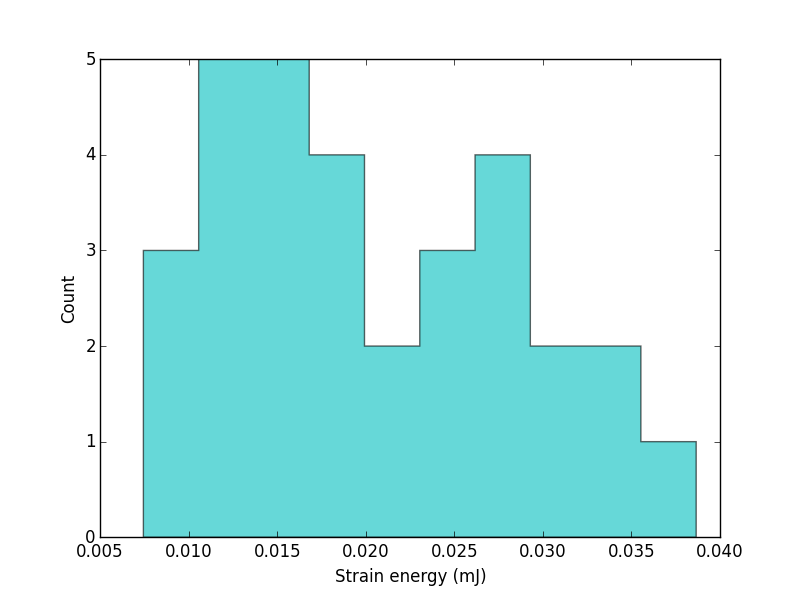
\includegraphics[width=\doubleimagewidth]{figures/fzk-w-histogram.png}
    \caption{Histogram of the absorbed strain energy at the moment of crushing for \lis~pebbles as measured in single pebble crush experiments.}
    \label{fig:fzk-w-hist}
\end{figure}

\begin{figure}
        \centering
        \begin{subfigure}[b]{\doubleimagewidth}
                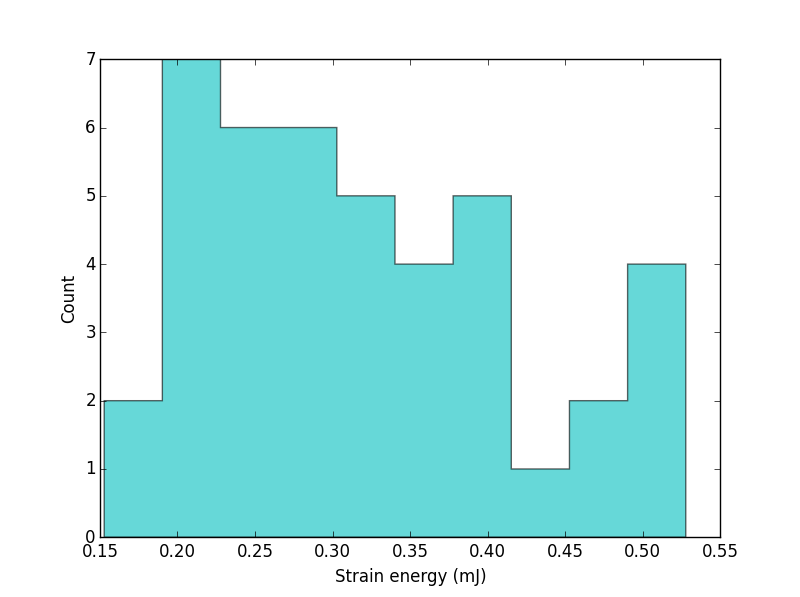
\includegraphics[width=\textwidth]{figures/nfri-1mm-w-histogram.png}
                \caption{$\bar{d}_p = 1$ mm}
                \label{fig:nfri-1-w-hist}
        \end{subfigure}
        ~
        \begin{subfigure}[b]{\doubleimagewidth}
                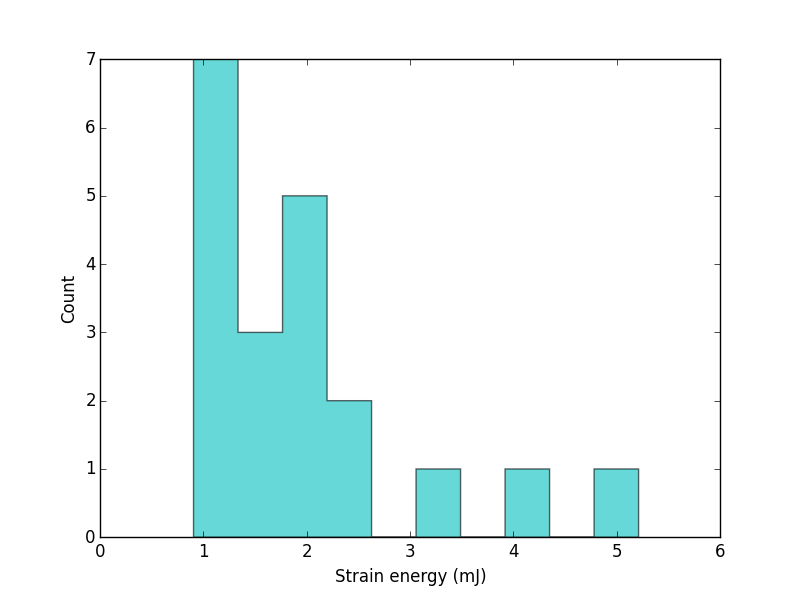
\includegraphics[width=\textwidth]{figures/nfri-1.5mm-w-histogram.png}
                \caption{$\bar{d}_p = 1.5$ mm}
                \label{fig:nfri-1.5-w-hist}
        \end{subfigure}
        \caption{Histogram of the absorbed strain energy at the moment of crushing for \lit~pebbles as measured in single pebble crush experiments.}\label{fig:nfri-w-hist}
\end{figure}

The normal force between two elastic objects is a function of the material properties of the interacting objects (see, \textit{e.g.}, \Cref{eq:hertz-normal-force}). We cannot, therefore, directly compare the forces between the pebble and test stand with pebble-pebble contacts in an ensemble. An approached used by some solid breeder researchers is to relate the total absorbed strain energy of the pebble.\cite{Zhao2013,Annabattula2012a}

Integrating the Hertzian force along the overlap of contact to find the strain energy $W_\epsilon$, of a given contact,
\begin{equation}\label{eq:strain-energy-integral}
	W_\epsilon = \int_0^{\delta_c}\!F_n(\delta')\,\mathrm{d}\delta'
\end{equation}
where the upper limit of the integration is the critical overlap $\delta_c$. Inserting the Hertzian relation of \Cref{eq:hertz-normal-force} into \Cref{eq:strain-energy-integral} gives,
\begin{align}
	W_\epsilon& = \int_0^{\delta_c}\!  \frac{4}{3}E^*\sqrt{R^*}\,\delta'^{3/2} \,\mathrm{d}\delta' \\
	%W_\epsilon & = \frac{4}{3}E^*\sqrt{R^*} \left[\frac{2}{5}\,{\delta_c}^{5/2}\right] \\
	W_\epsilon & = \frac{8}{15}E^*\sqrt{R^*}\, {\delta_c}^{5/2}
\end{align}

I will call the strain energy of the pebble compressed between platens as the lab strain energy, $W_{\epsilon,L}$. In pebble crushing experiments, we record the strain energy absorbed up to the point of crushing, the data for \lis~and \lit~pebbles are shown in Figs.~\ref{fig:fzk-w-hist} and~\ref{fig:nfri-w-hist}, respectively. The strain energy of two particles in contact will be $W_{\epsilon,B}$. The assumption is made that, if each contact interaction is integrated to the proper critical overlap, the strain energies will be equal at that contact. The critical lab value is equated to the ensemble value,
\begin{equation}
	W_{\epsilon,L} = W_{\epsilon,B} = \frac{8}{15}E_B^*\sqrt{R_B^*}\, {\delta_{c,B}}^{5/2}
\end{equation}
which allows one to solve for the interacting pebble bed overlap as a function of the lab strain energy,
\begin{equation}
	\delta_{c,B} = \left[\frac{15W_{\epsilon,L}}{8E_B^*\sqrt{R_B^*}}\right]^{2/5}
\end{equation}

This overlap can be reinserted to the Hertz force of \Cref{eq:hertz-normal-force} to find the critical force (crush force) of the interacting particles in the numeric ensemble as a function of the critical strain energy of the lab. Doing this, we find,
\begin{equation}\label{eq:peb_hertz}
	F_{c,B} = C{E_B^*}^{2/5}{R_B^*}^{1/5}W_{\epsilon,L}^{3/5}
\end{equation}
where $C = \frac{4}{3}\left(\frac{15}{8}\right)^{3/5}$.

Equation~\ref{eq:peb_hertz} is a generic translation between lab materials and packed bed materials. We will use the equation as the basis for our pebble crushing prediction in DEM simulations. Before implementing a custom crush-predicting method into the DEM code, I will review other attempts at modeling and predicting crush behavior in packed beds.





%~~~~~~~~~~~~~~~~~~~~~~~~~~~~~~~~~~~~~~~~~~~~~~~~~~~~~~~~~~~~~~~~~~~~~~~~~~~~~~~~~~~~~~~~~~~~~~~~~~~~~~~~~~~
% new subsection
%~~~~~~~~~~~~~~~~~~~~~~~~~~~~~~~~~~~~~~~~~~~~~~~~~~~~~~~~~~~~~~~~~~~~~~~~~~~~~~~~~~~~~~~~~~~~~~~~~~~~~~~~~~~
\subsection{Calculating Critical Strain Energy}
With the rise of micro-mechanical tools and computing power, attempting to predict when ceramic pebbles will crush in an ensemble, based on inter-particle contact forces, has received considerable attention. In this section I review literature studying granular crushing.

Probability and statistics were applied to the study of packed beds of brittle grains by Marketos and Bolton\cite{Marketos2007}. The fundamental assumption in their predictive method was the independence of crushing events. They used their model to predict the initiation of crushing as well as the evolution of the packing after crushing. They created somewhat arbitrary probability distributions of the strength of their granular particles,
\begin{equation}
	h(\Phi) = \frac{0.0395}{\sqrt{\Phi}}
\end{equation}
where $\Phi$ is a characteristic strength parameter falling between 160 and 640~N. The form of their distribution was based on single crushing tests on quartz particles from Nakata\etal.

A common alternative distribution is to use a form first proposed by Weibull for a material under uniform stress\cite{Kwok2013,Zhao2011,nakata1999probabilistic,Zhao2013,Pitchumani2004}. The form, as written by Zhao\etal~is,
\begin{equation}
	P_s = 1 - \exp\left[-\left(\frac{W_c}{W_\text{mat}}\right)^m\right]
\end{equation}
where $W_c$ is the energy absorbed by the pebble and $W_\text{mat}$ and $m$ characterize the material. An important note is how to calculate the critical strain energy for the pebble. Refs.~\cite{Marketos2007} and \cite{Zhao2011} note the necessity to consider the coordination number dependence on total strain energy. In other words, the total strain energy is the cumulative total of strain energy at every contact. Zhao\etal~give the critical strain as
\begin{equation}
	W_c = \sum_{i=1}^{Z_i}\left(\frac{9}{80 R_{ij}^*}\right)^{1/3} \left(\frac{1}{E_{ij}^*}\right)^{2/3} F_{n,ij}^{5/3}
\end{equation}
where $Z$ is the coordination number of pebble $i$. 

However, Russell\etal, analyzed simple, ideal granular assemblies for which they could find analytical solutions to stress distributions inside of pebbles.\cite{Russell2009} In their work, failure of a granular particle initiates at the location of maximum of the stress invariant ratios. In the contact of elastic spheres, the stress fields near the contact areas are highly localized. Because of the highly localized effects, Russell\etal~find that in granular assemblies the contributions to failure initiation are not additive. They discovered that the initiation of failure is always located adjacent to the largest force irrespective of the material properties or geometric size of the pebbles in an ensemble. Russell\etal conclude: \emph{the largest contact force acting upon a particle is the primary agent driving the damage of the individual}.\cite{Russell2009} Based upon the failure criterion developed for brittle materials, crushing of an individual does not directly depend upon the presence or magnitude of any lesser contact forces acting on the particle or the material properties of the particle. Although their results were obtained for idealized assemblies, the results are generally true for any situation where multiple contact forces are present.

\begin{figure}[!t]
\centering
    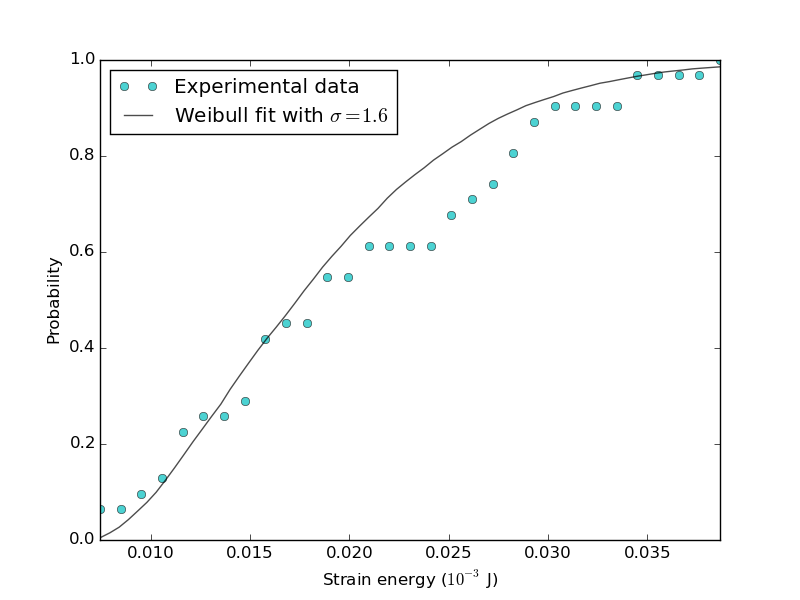
\includegraphics[width=\doubleimagewidth]{figures/fzk-w-cdf-fit.png}
    \caption{Fitting the strain energy with a Weibull distribution with shape parameter specific for the \lis~pebbles.}
    \label{fig:fzk-w-cdf}
\end{figure}

\begin{figure}
        \centering
        \begin{subfigure}[b]{\doubleimagewidth}
                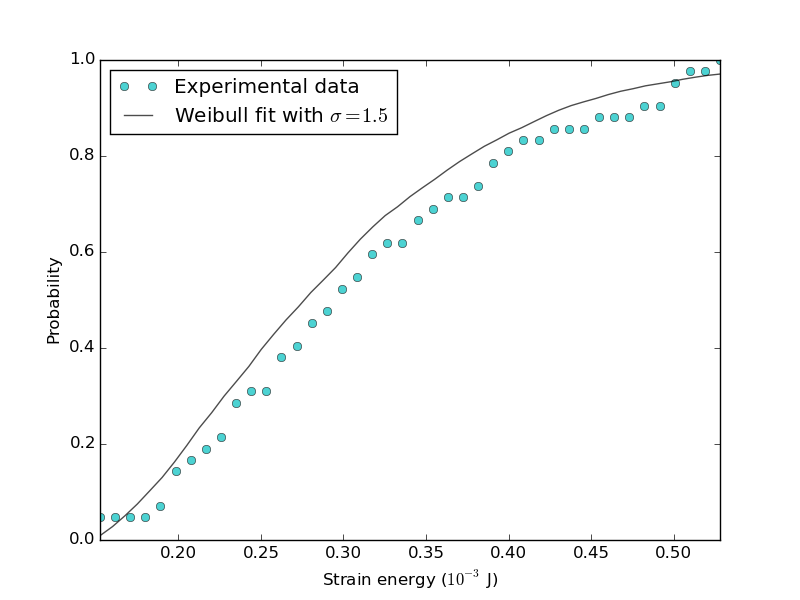
\includegraphics[width=\textwidth]{figures/nfri-1mm-w-cdf-fit.png}
                \caption{$\bar{d}_p = 1$ mm}
                \label{fig:nfri-1-w-cdf}
        \end{subfigure}
        ~
        \begin{subfigure}[b]{\doubleimagewidth}
                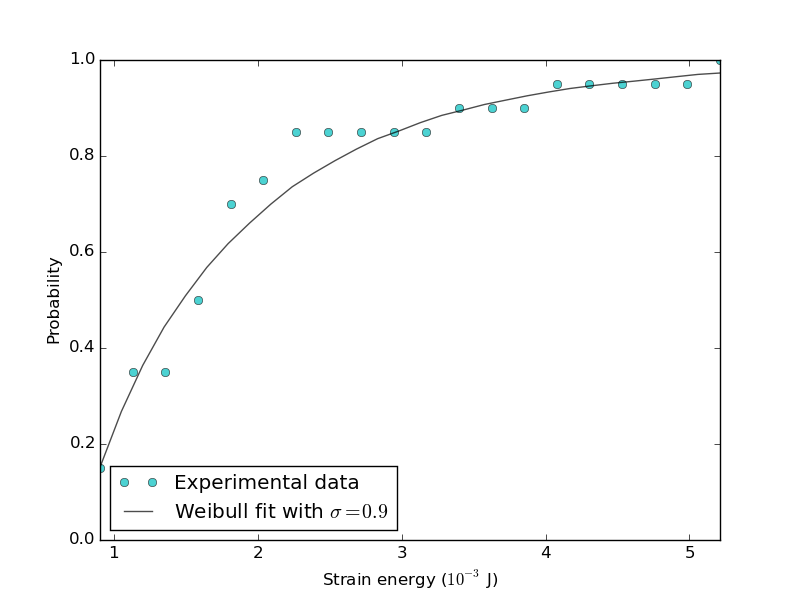
\includegraphics[width=\textwidth]{figures/nfri-1.5mm-w-cdf-fit.png}
                \caption{$\bar{d}_p = 1.5$ mm}
                \label{fig:nfri-1.5-w-cdf}
        \end{subfigure}
        \caption{Fitting the strain energy with a Weibull distribution with shape parameter specific for the two batches of \lit~pebbles.}\label{fig:nfri-w-cdf}
\end{figure}

Based on the compelling arguments of Russell\etal, I define a critical force as the maximum contact force on the pebble in our assembly,
\begin{equation}
	F_{c} = \max F_{n,ij}
\end{equation}

Then define a pebble crushing event as occurring when \textit{any} force on the pebble in the bed is greater than the critical bed force defined from \Cref{eq:peb_hertz},
\begin{equation}\label{eq:crush-predict}
  F_{c} > F_{c,B} = \frac{4}{3}\left(\frac{15}{8}\right)^{3/5}{E_B^*}^{2/5}{R_B^*}^{1/5}W_{\epsilon,L}^{3/5}
\end{equation}

In the implementation into DEM, the probabilistic features appear naturally in this formulation from the measured $W_{\epsilon,L}$ of experiments. This value follows a probability distribution and therefore imparts a distribution shape to the $F_{c,B}$ prediction. Cumulative distribution functions are generated for the strain energy data (see Fig.~\ref{fig:nfri-w-hist}). From that data, we fit Weibull distribution curves, of the form
\begin{equation}
	\Xi = \lambda\left[-\ln(W_\epsilon)\right]^{1/\sigma}
\end{equation}
where the shape parameter, $\sigma$, is fit to the specific curve of each set of experimental data and the second parameter, $\lambda$ is defined as
\[
\lambda = \bar{W}_\epsilon - \min W_\epsilon
\]

In Figs.~\ref{fig:fzk-w-cdf} and~\ref{fig:nfri-w-cdf} we see the experimental data and the Weibull fits specific to the ceramic material and batch. The Weibull distribution functions are recreated numerically in the assignment of each pebbles `critical bed force' value.


% \cite{Hiramatsu1966}
% From , 
% \begin{align*}
% \sigma_{cr} = \cfrac{2.8}{\pi}\cfrac{F_{cr}}{4R^2}
% \end{align*}
Research on pebble damage has been taken up by others in the fusion community to predict the onset of pebble crushing as a function of an external pressure and the resulting changes to mechanical properties such as the stress-strain of the pebble bed.\cite{Annabattula2012a, Zhao2012, Zhao2013} Other fields of engineering have also employed DEM in studies of granular crushing with generally similar modeling approaches.\cite{Marketos2007,Pitchumani2004}


In modeling pebble damage, there are two main tasks: predicting when the grain crushes and what happens to the pebble during the crushing event. For the former, the task is to develop a model for predicting a pebble crushing event; \textit{i.e.} what external load (mechanical or thermal) will cause a pebble to crack, shatter, fracture, etc. To tackle the latter is to develop a model which simulates the damage of that pebble; \textit{i.e.} a scheme to treat a cracked, shattered, or crushed pebble in the assembly as small particles, removed particles, or particles with modified material properties.

\begin{figure}[!t]
\centering
	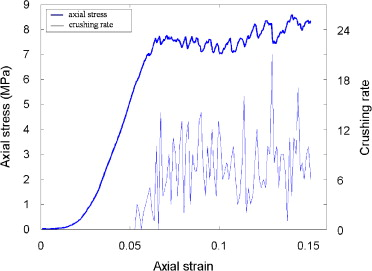
\includegraphics[width=\singleimagewidth]{figures/markets-bolton-stress-strain-crushing.jpg}
	\caption{Stress-strain response of a pebble bed with crushed pebbles. Reproduced from Ref.~\cite{Marketos2007}}
	\label{fig:marketos-bolton-stress-strain}
\end{figure}

\begin{figure}[!t]
\centering
	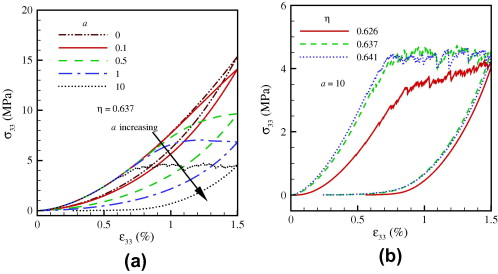
\includegraphics[width=\singleimagewidth]{figures/annabattula-stress-strain-crushing.jpg}
	\caption{Stress-strain response of a pebble bed with crushed pebbles. Reproduced from Ref.~\cite{Annabattula2012a}}
	\label{fig:annabattula-stress-strain}
\end{figure}

The numerical study to follow will focus on the `what happens' question. In work by Marketos and Bolton, they treated a crushed pebble very similar to Van Lew\etal; when a pebble was damaged it was removed completely from the assembly.\cite{Marketos2007,VanLew2014} Marketos and Bolton study the stress-strain response of a pebble bed with a predictive crushing routine while Van Lew\etal~studied the effective thermal conductivity of a damaged pebble bed.

However, in the case of Van Lew\etal, the technique of removing a pebble is limited by the fact that energy input into two systems being studied is not comparable. Because of volumetric energy deposition in the simulations, the total energy pouring into the non-damaged system would be
\begin{equation}
	E_h = \frac{q'''_\text{nuc} V_\text{peb} N}{V_\text{bed}}
\end{equation}
where $N$ is the total number of pebbles of volume $V_\text{peb}$ that exist in the pebble bed of volume $V_\text{bed}$. After a crushing event, when pebbles are removed, the total amount of energy is
\begin{equation}
	E_h' = \frac{q'''_\text{nuc} V_\text{peb} \eta N}{V_\text{bed}}
\end{equation}
where $\eta$ is the percent of crushed pebbles. Obviously then, the ratio of the two heating rates is\begin{equation}
	\frac{E_h'}{E_h} = 1 - \eta
\end{equation}
and the energy deposited is not balanced between a virgin bed and one with crushed pebbles. We will attempt to address this issue.

\subsection{Modeling Fragments of a Crushed Pebble}\label{sec:fragmentation}
In the DEM framework, we are limited to modeling elastic spheres. If we strictly wish to conserve mass between a solid pebble of radius $R_p$ and the crushed fragments of radius $R_c$, then the number of crushed fragments (spheres) per crushed pebble is
\begin{equation}\label{eq:nc-crushed-fragments}
	N_c = \left(\frac{R_c}{R_p}\right)^{-3}
\end{equation}

Thus the number of fragments goes like the inverse of radius ratio to the third power and the number of crushed fragments to represent a single crushed pebble increases rapidly as the fragments shrink. The relationship between radius ratio and number of fragment particles is given in Fig.~\ref{fig:fragment-count}. Note that in the DEM simulation, it is impossible to insert fractions of a particle so the number of fragment pebbles is rounded to the nearest integer in the figure.


\begin {table}[htp] %
\caption{Example values of the particle crush fragments, $N_c$, necessary to replace a single crushed particle and obey conservation of mass (fragment number is rounded to nearest integer).}
\label {tab:rstar-Nc} \centering %
\begin {tabular}{ S[table-format=3.2]S[table-format=3.2] }
\toprule
$R_c/R_p$ 						& $N_c$  				\\\otoprule
0.20                            & 125                   \\    
0.30                            & 37               \\
0.40                            & 16                   \\
0.50                            & 8                         \\
0.75                            & 2                \\\bottomrule
\end{tabular}
\end{table}



\begin{figure}[!t]
\centering
    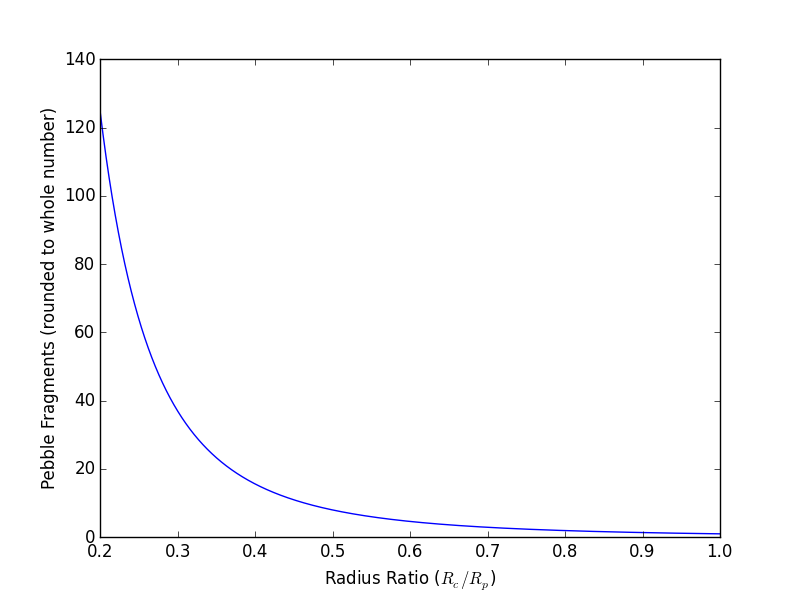
\includegraphics[width=\singleimagewidth]{figures/crush-fragments/pebble-fragment-count.png}
    \caption{Number of fragment pebbles necessary to conserve mass increases rapidly as the size of the radius ratio ($\frac{R_c}{R_p}$) decreases.}
    \label{fig:fragment-count}
\end{figure}

In typical DEM simulations that can run within reasonable amounts of time on the machines available for this dissertation, a reasonable number of particles is on the order of \num{10000}. Significantly more and the run times become impractical for study. To show how quickly the number of particle fragments can quickly get out of hand in a simulation with small $R_c/R_p$, if we begin with \num{6000} pebbles and only 2\% break, with a radius ratio of $R_c/R_p = 0.2$, the number of pebbles to be added would be \num{15000}. The new particle fragments (less the crushed particles) plus the original would require \num{21000} particles in the system. In our simulations, we often test the effects on effective thermal conductivity at particle crush amounts of to 10\%. For the pebble bed mentioned here, that would mean \num{81000} particles in the system and it would be computationally taxing. The result is that, for the sake of computational times, the larger crush fragment radii are desired, \textit{i.e.} $R_c/R_p > 0.3$.

However, aside from satisfying conservation of mass, we must physically insert the particle fragments into void space in the simulation domain. During the course of the simulation, when we choose to replace the pebble with the fragments, the only available room is the spherical void left over by the damaged pebble. Thus a constraint is the smallest sized sphere that will allow the given spheres at most dense packing. 

Dense packing of spheres inside a larger sphere is an interesting mathematical problem. \href{http://www.randomwalk.de/sphere/insphr/spisbest.txt}{Hugh Pfoertner} keeps a compiled list of many solutions for a number of particles; many solutions are his are from Gensane.\cite{gensane2003dense} If we consider, for instance, that a radius ratio of $R_c/R_p = 0.3$ requires 37 particle fragments, then we can also find from Ref.~\cite{gensane2003dense} that 37 particles would have to be of radius 0.2406866 to fit into a single sphere of radius of unity. We defined the particle fragment radius as $R_c$, the original particle as $R_p$, and then the radius of sphere necessary to hold the $N_c$ fragments will be $R_N$, we can find a relationship between the volume of sphere $V_p$ and necessary volume $V_N$,
\begin{equation}
	r_1^* = \frac{R_c}{R_p}
\end{equation}
and
\begin{equation}
	r_2^* = \frac{R_c}{R_N}
\end{equation}
then 
\begin{equation}
	R_N = R_p \frac{r_1^*}{r_2^*}
\end{equation}
thus
\begin{equation}
	\frac{V_N}{V_p} = \left(\frac{r_1^*}{r_2^*}\right)^3
\end{equation}

If we choose a linearly spaced distribution of $r_1^*$ between 0 and 1, we can then find how many $N_c$ particles are necessary to conserve mass, then from the $N_c$ particles we can find from the database of sphere packing solutions the size of sphere that would be necessary to fit the $N_c$ particles. The calculations are carried out and shown in Fig.\ref{fig:volume-ratio}. The data in Ref.~\cite{gensane2003dense} does not go above 72 spheres so we are limited to radius ratios above about $r_1^* > 0.24$.

The plot of Fig.\ref{fig:volume-ratio} shows that for particle fragments of reasonable numbers ($N_c\approx 20$ for $r_1^*\approx 0.3$), the volume necessary to fit the number of volume-conserving particles is greater than double the volume of the original sphere! Therefore from the point of view of having the physical space to insert the fragments, smaller sized fragments are ideal. To insert the few number of large particles would require disrupting the packing in the region of the damaged particle.

Thus we have competing results from the two requirements. Computationally, we desire larger crushed fragments yet we need smaller fragments in order to fit them into the system in a non-disruptive way.

\begin{figure}[!t]
\centering
    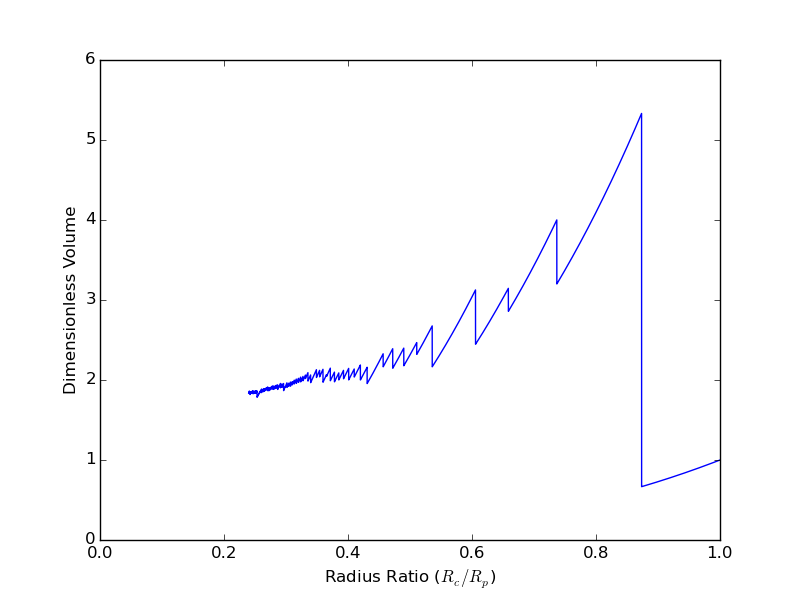
\includegraphics[width=\singleimagewidth]{figures/crush-fragments/fragment-volume-ratio.png}
    \caption{The volume necessary to house the particles of different radius ratios decreases toward unity as the radius ratio decreases. It is greater than 5 times the volume for large $r_1^*$.}
    \label{fig:volume-ratio}
\end{figure}


\begin{figure}[!ht]
	\centering
	\begin{subfigure}[b]{\doubleimagewidth}
		\centering
		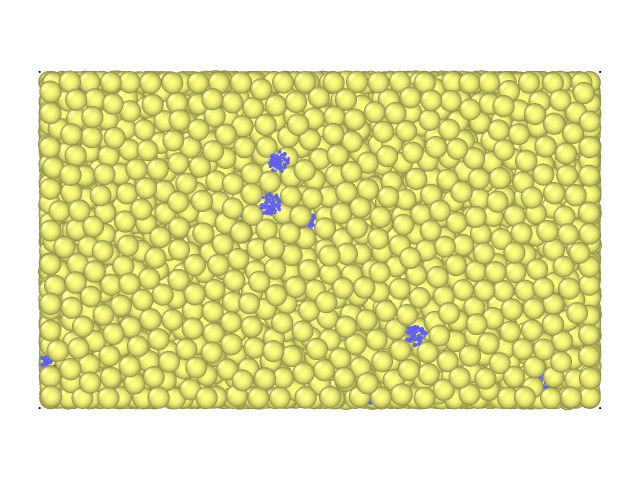
\includegraphics[width=\textwidth]{figures/crush-fragments/0.20-1.png}
		\caption{initial}
	\end{subfigure}
	\begin{subfigure}[b]{\doubleimagewidth}
		\centering
		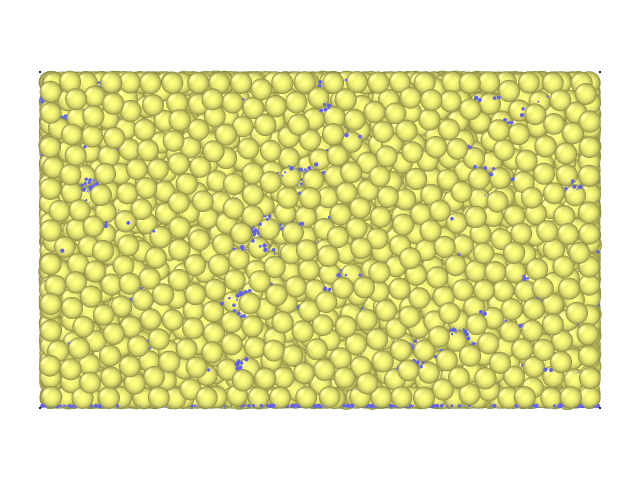
\includegraphics[width=\textwidth]{figures/crush-fragments/0.20-2.png}
		\caption{final}
	\end{subfigure}
	\caption{$N_c = 8594$, $N_\text{tot} = 15430$, $r_1^* = 0.20$. Side view of the packing arrangement and settling for different crush fragment sizes. The small crush fragments migrate far through the height of the bed. The yellow particles are the original pebbles and the blue are fragments inserted into the system after pebble crushing.}
\label{fig:crush-settling-pictures-1}
\end{figure}
\begin{figure}[!ht]
	\begin{subfigure}[b]{\doubleimagewidth}
		\centering
		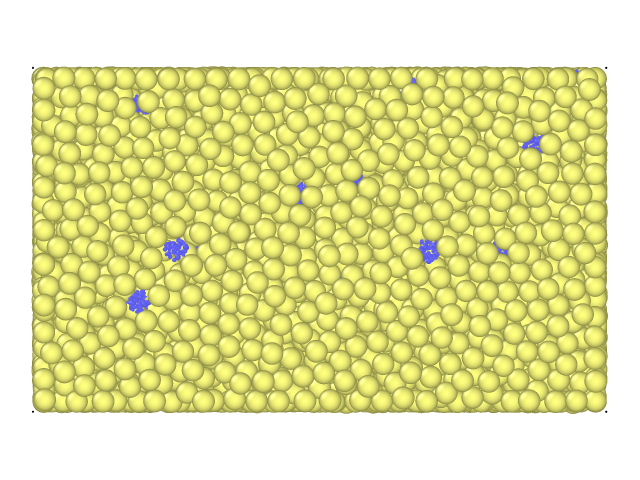
\includegraphics[width=\textwidth]{figures/crush-fragments/0.25-1.png}
		\caption{initial}
	\end{subfigure}
	\begin{subfigure}[b]{\doubleimagewidth}
		\centering
		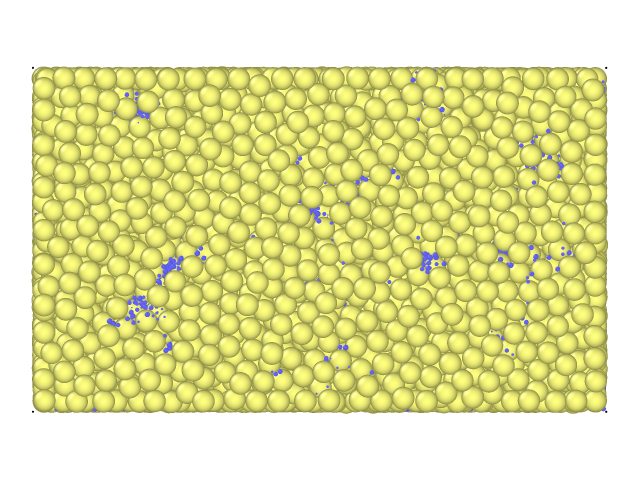
\includegraphics[width=\textwidth]{figures/crush-fragments/0.25-2.png}
		\caption{final}
	\end{subfigure}
	\caption{$N_c = 4400$, $N_\text{tot} = 11222$, $r_1^* = 0.25$. Side view of the packing arrangement and settling for different crush fragment sizes. The small crush fragments migrate far through the height of the bed. The yellow particles are the original pebbles and the blue are fragments inserted into the system after pebble crushing.}
\label{fig:crush-settling-pictures-2}
\end{figure}

\begin{figure}[!ht]
	\centering
	\begin{subfigure}[b]{\doubleimagewidth}
		\centering
		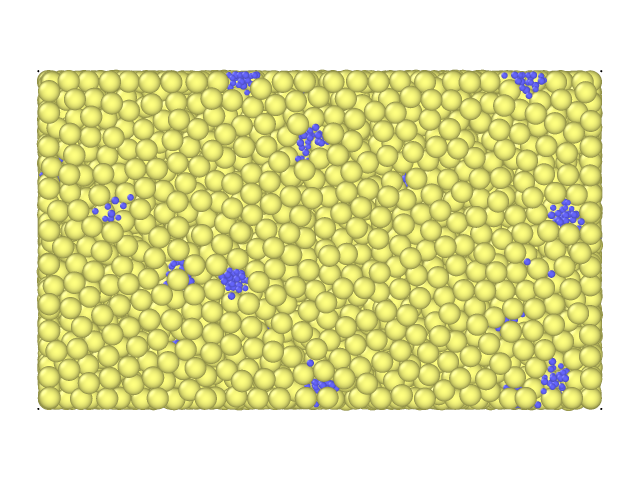
\includegraphics[width=\textwidth]{figures/crush-fragments/0.35-1.png}
		\caption{initial}
	\end{subfigure}
	\begin{subfigure}[b]{\doubleimagewidth}
		\centering
		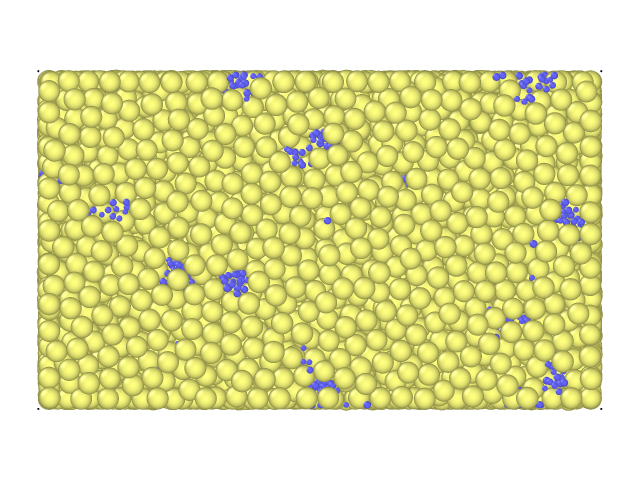
\includegraphics[width=\textwidth]{figures/crush-fragments/0.35-2.png}
		\caption{final}
	\end{subfigure}
	\caption{$N_c = 1603$, $N_\text{tot} = 8393$, $r_1^* = 0.35$. Side view of the packing arrangement and settling for different crush fragment sizes. The bigger fragments remain largely in place. The yellow particles are the original pebbles and the blue are fragments inserted into the system after pebble crushing.}
\label{fig:crush-settling-pictures-3}
\end{figure}
\begin{figure}[!ht]
	\begin{subfigure}[b]{\doubleimagewidth}
		\centering
		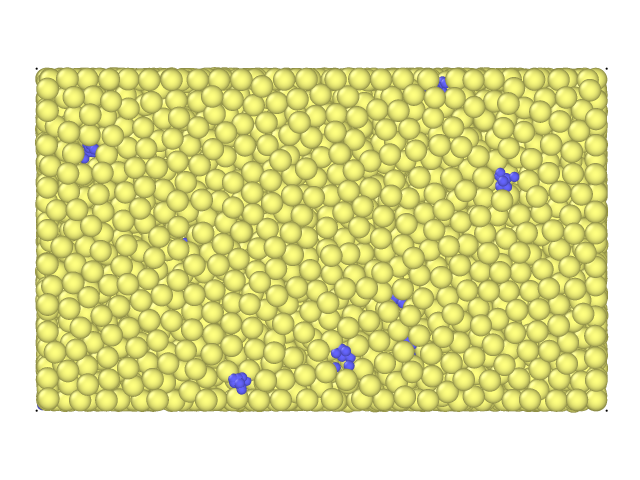
\includegraphics[width=\textwidth]{figures/crush-fragments/0.50-1.png}
		\caption{initial}
	\end{subfigure}
	\begin{subfigure}[b]{\doubleimagewidth}
		\centering
		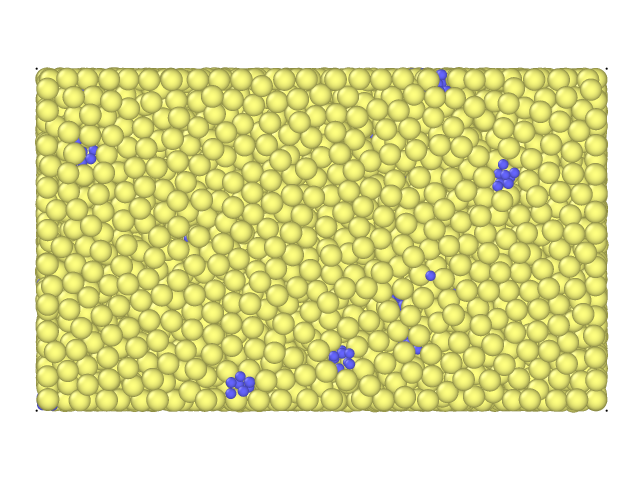
\includegraphics[width=\textwidth]{figures/crush-fragments/0.50-2.png}
		\caption{final}
	\end{subfigure}
	\caption{$N_c = 550$, $N_\text{tot} = 7358$, $r_1^* = 0.50$. Side view of the packing arrangement and settling for different crush fragment sizes. The bigger fragments remain largely in place. The yellow particles are the original pebbles and the blue are fragments inserted into the system after pebble crushing.}
\label{fig:crush-settling-pictures-4}
\end{figure}
\FloatBarrier

To study the effects on a pebble bed of different fragmentation schemes, I begin with a bed of \num{6875} particles and randomly crush 1\%. This was done with a range of fragments of size $r_1^* = [0.20, 0.25, 0.35, 0.50]$. The number of particles inserted for these different $r_1^*$ followed the from \Cref{eq:nc-crushed-fragments}. In the images of Figs.~\ref{fig:crush-settling-pictures-1},~\ref{fig:crush-settling-pictures-2},~\ref{fig:crush-settling-pictures-3}, and~\ref{fig:crush-settling-pictures-4}, we see the initial packing of new particle fragments (in blue) settle into the interstitial gaps of the packing structure of original pebbles (yellow).

\begin{figure}[!t]
\centering
    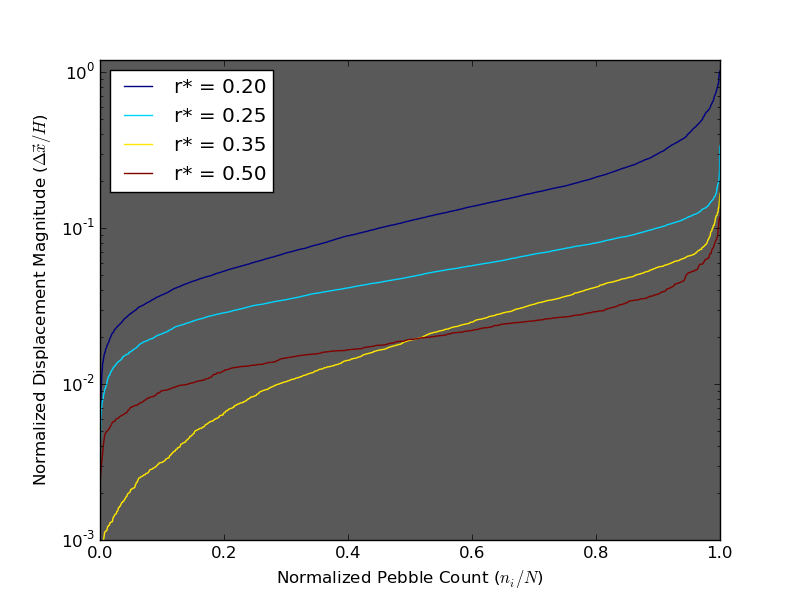
\includegraphics[width=\singleimagewidth]{figures/crush-fragments/displacement-scatter-radius-ratios.png}
    \caption{After the particle fragments are inserted into the system they re-settle due to gravity and inter-particle forces. The small fragments travel much further throughout the bed than the large fragments.}
    \label{fig:displacement-scatter}
\end{figure}

The settling of crushing fragments is also visualized in Fig.~\ref{fig:displacement-scatter}. For this figure, the magnitude of displacement for all the crushed fragments is recorded based on the change between initial insertion location and final resting place. The displacement of the fragments is normalized against the height of the pebble bed, $H$. The fragments with $r_1^* = 0.2$ are seen to travel, on average, 10\% of the height of the pebble bed before coming to rest; some of them travel more than the entire height of the bed -- as if in a game of Plinko. In contrast, the particle fragments of size $r_1^* = 0.35$ and $r_1^* = 0.5$ travel only about 1\% of the height of the bed before coming to rest. 

\begin{figure}[!t]
\centering
    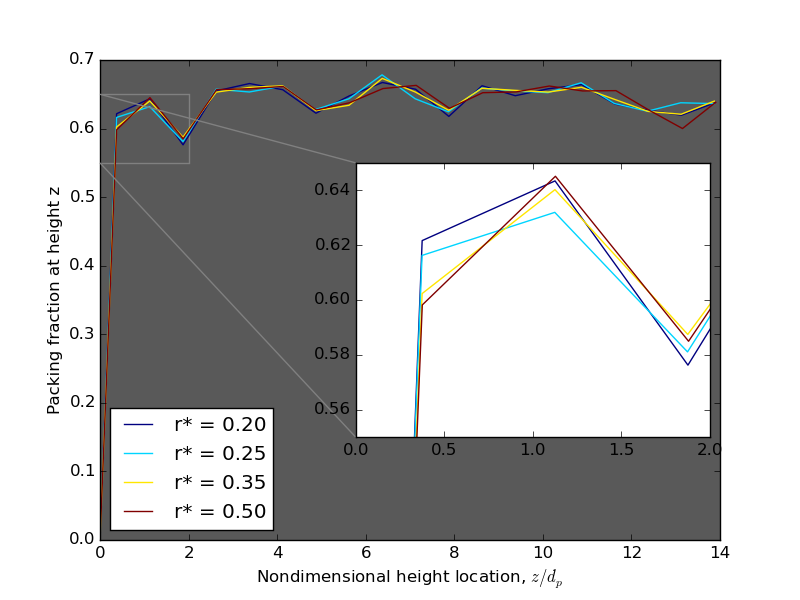
\includegraphics[width=\singleimagewidth]{figures/crush-fragments/packing-fraction-height.png}
    \caption{For only 1\% of crushed pebbles, the re-settling of small pebble fragments has a small effect on the overall packing fraction of the pebble bed. In the inset, the main influence is seen in the slight increase of packing fraction within the first pebble radius of the floor.}
    \label{fig:fragment-packing-fraction}
\end{figure}

From Fig.~\ref{fig:displacement-scatter}, the impression then arises that the large displacement magnitudes of the small crush fragments would result in an overall less-dense bed with large increase in packing fraction near the floor where pebbles settle. For 1\% crushed pebbles, there is some observable changes to the local packing fraction near the floor of the pebble bed, but no appreciable changes elsewhere in the bulk. In Fig.~\ref{fig:fragment-packing-fraction}, the packing fractions of the four different pebble beds are given. We look closely at the distribution within the first pebble diameter (see inset of Fig.~\ref{fig:fragment-packing-fraction}) and see the small crush fragments have a small change to the local packing fraction as they settled onto the floor of the container. Simulations can be run with a greater percentage of failed pebbles to discern more clearly the settling impact on local packing fractions. This is discussed in the Remaining Work section.


\begin{figure}[!ht]
	\centering
	\begin{subfigure}[b]{\doubleimagewidth}
		\centering
		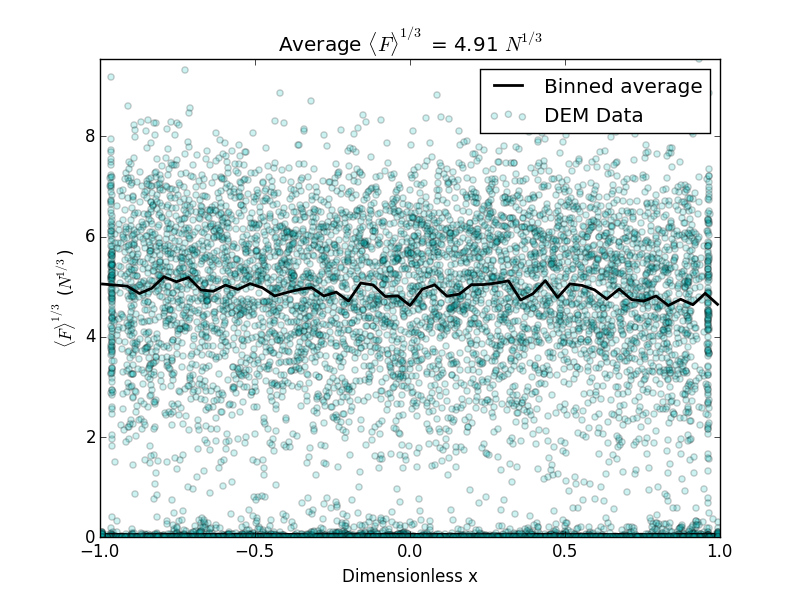
\includegraphics[width=\textwidth]{figures/crush-fragments/force-scatter-20.png}
		\caption{$r_1^* = 0.20$}\label{fig:fragment-contact-forces-20}
	\end{subfigure}
	\begin{subfigure}[b]{\doubleimagewidth}
		\centering
		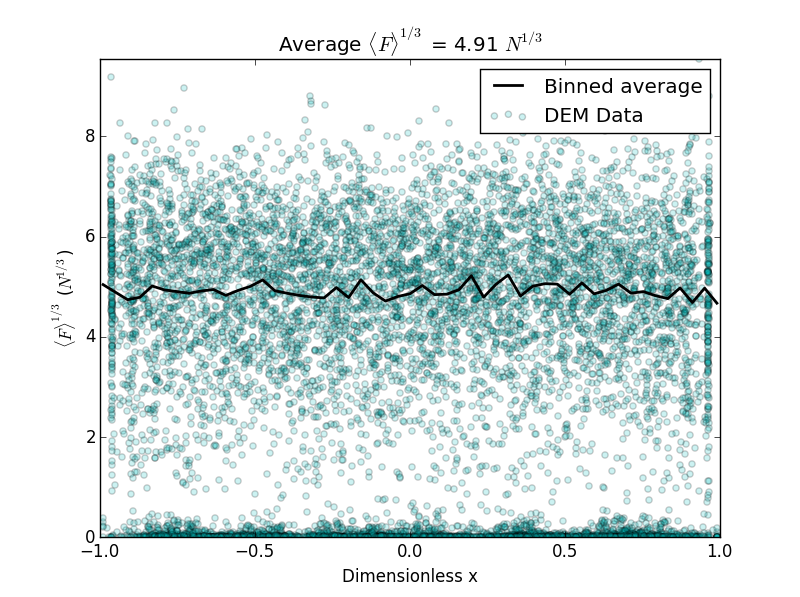
\includegraphics[width=\textwidth]{figures/crush-fragments/force-scatter-25.png}
		\caption{$r_1^* = 0.25$}\label{fig:fragment-contact-forces-25}
	\end{subfigure}

	\begin{subfigure}[b]{\doubleimagewidth}
		\centering
		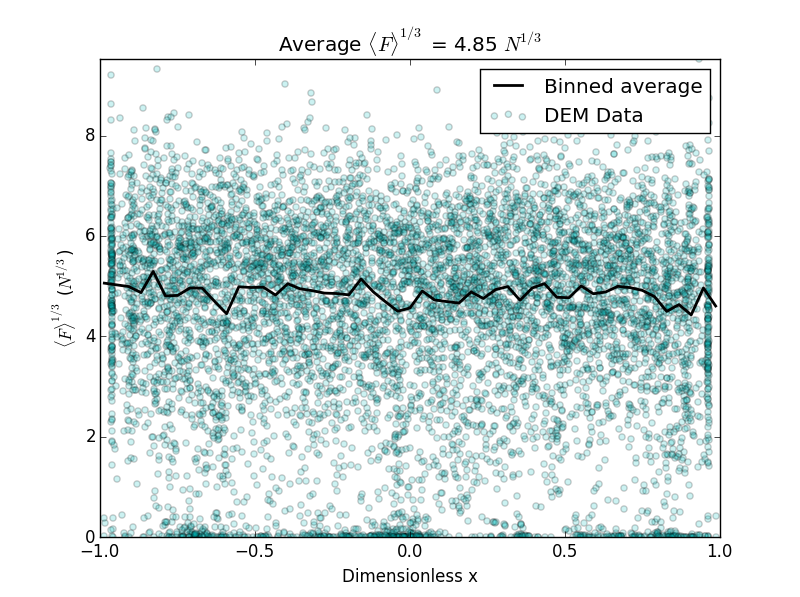
\includegraphics[width=\textwidth]{figures/crush-fragments/force-scatter-35.png}
		\caption{$r_1^* = 0.35$}
	\end{subfigure}
	\begin{subfigure}[b]{\doubleimagewidth}
		\centering
		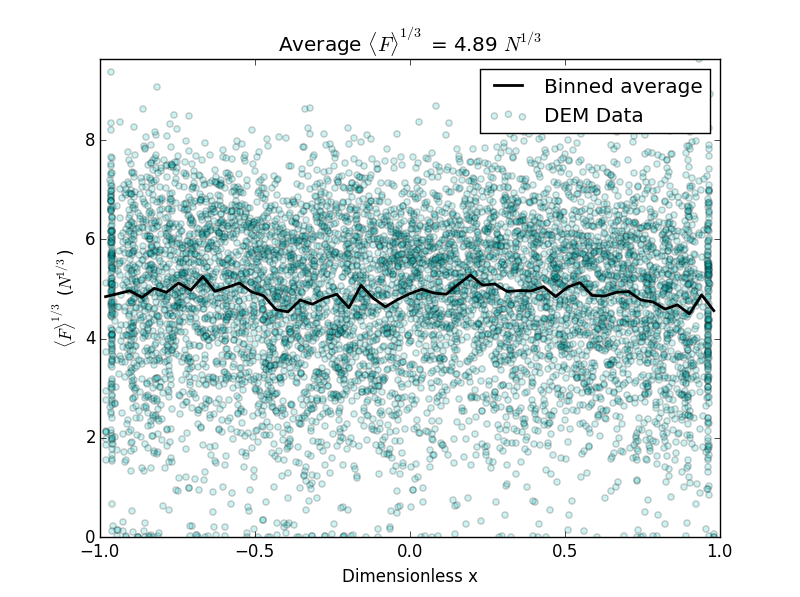
\includegraphics[width=\textwidth]{figures/crush-fragments/force-scatter-50.png}
		\caption{$r_1^* = 0.50$}
	\end{subfigure}
	\caption{Contact force distributions throughout the pebble beds with different crush fragment sizes. Average forces in the bed are largely unaffected by the size of crushed particle fragments.}
\label{fig:fragment-contact-forces}
\end{figure}

\FloatBarrier

The last point to discuss is how the different size particles change the distribution of contact forces inside the ensemble. We plot the scatter of contact forces for all the pebbles in the ensemble in Fig.~\ref{fig:fragment-contact-forces}. We are most interested in the contact loads carried by the large particles that make up the force network after crush fragments are inserted into the ensemble. The small fragments, moving through the interstitial gaps, are not expected to carry much load. Therefore in the data processing for the subplot of Figs.~\ref{fig:fragment-contact-forces-20} and~\ref{fig:fragment-contact-forces-25}, I did not include the vast number of small forces on the fragments in the average value of contact force. Opposingly, the larger fragments, $r_1^*>0.4$, are expected to be inserted firmly into the contact network and their contribution to the average value is included.

What we see in Fig.~\ref{fig:fragment-contact-forces} is that the average contact forces in the pebble bed remain mostly unchanged as a function of the size of the fragment radii. For all pebble beds, after the bed re-settles from the crushing event, the average contact forces (to the 1/3 power, which is the value important for heat transfer, see \cref{sec:dem-studies-effective-conductivity}) are approximately $4.9\ N^{1/3}$. None of the beds have a maximum value greater than $9\ N^{1/3}$.



%~~~~~~~~~~~~~~~~~~~~~~~~~~~~~~~~~~~~~~~~~~~~~~~~~~~~~~~~~~~~~~~~~~~~~~~~~~~~~~~~~~~~~~~~~~~~~~~~~~~~~~~~~~~
% new subsection
%~~~~~~~~~~~~~~~~~~~~~~~~~~~~~~~~~~~~~~~~~~~~~~~~~~~~~~~~~~~~~~~~~~~~~~~~~~~~~~~~~~~~~~~~~~~~~~~~~~~~~~~~~~~
\subsection{Conclusions of Pebble Failure Modeling}

This section began with a means of translating the measurements of force-travel and crushing results of experimental data on individual pebbles to the force of contacts between particles in an ensemble. The parameter acting as translator was a critical strain energy value, an integral of the force-displacement of a contact in either reference (lab or ensemble). I then discussed the philosophy and reasoning behind a crush-predicting criteria I have implemented into DEM code for flagging a crushing event based on measurements of contact forces on pebbles in the ensemble. In short, I consider \textit{only the single largest contact force} on a pebble, irrespective of the number and magnitude of lesser contact forces on that pebble when predicting a crush event. The probabilistic nature of experimental measurements is naturally incorporated into the numeric computations via recreations of the probability distribution functions matched to experimental measurements of strain energy.

I also introduced a method for introducing crushed pebble fragments into an ensemble after pebble damage is predicted via the above criteria. The method was necessary to enforce conservation of mass between pebble beds before and after the crushing event which is necessary for also balancing the energy deposition into the bed from volumetric heating before and after the crushing event. We then showed that fragments increase the computational time as $(1/r_1^*)^{1/3}$ while the necessary minimum volume for inserting the particles follows roughly as $(r_1^*)^{1/3}$. The size of fragments may still influence the overall transport of energy in the system but in terms of localizing heat deposition due to settling fragments in interstitial regions, I also showed that the local packing fraction was changed very little over the range of radius ratios tested. Thus from the point of view of capturing proper thermophysics of the system, there does not seem to be a strict sensitivity to choice of radius ratio of fragmentations.



 


%%%%%%%%%%%%%%%%%%%%%%%%%%%%%%%%%%%%%%%%%%%%%%%%%%%%%%%%%%%%%%%%%%%%%%%%%%%%%%%%%%%%%%%%%%%%%%%%%%%%%%%%%%%%
%%%%%%%%%%%%%%%%%%%%%%%%%%%%%%%%%%%%%%%%%%%%%%%%%%%%%%%%%%%%%%%%%%%%%%%%%%%%%%%%%%%%%%%%%%%%%%%%%%%%%%%%%%%%
%
% new section
%
%%%%%%%%%%%%%%%%%%%%%%%%%%%%%%%%%%%%%%%%%%%%%%%%%%%%%%%%%%%%%%%%%%%%%%%%%%%%%%%%%%%%%%%%%%%%%%%%%%%%%%%%%%%%
%%%%%%%%%%%%%%%%%%%%%%%%%%%%%%%%%%%%%%%%%%%%%%%%%%%%%%%%%%%%%%%%%%%%%%%%%%%%%%%%%%%%%%%%%%%%%%%%%%%%%%%%%%%%
\section{Summary of DEM Modeling Development}

In the preceding sections I introduced the philosophy behind choosing the discrete element method as a tool for researching ceramic pebble beds for solid breeders, the basic governing equations of the discrete element method, and a number of enhancements to the technique based on observations performed at UCLA on individual ceramic pebbles.

Among the contributions to the field of DE modeling for ceramic breeders, a modified Young's modulus (fit to a probabilistic distribution) is shown to be necessary to capture the observed scatter of elasticity of ceramic pebbles. The modified Young's Modulus is realized in DEM simulations with a numeric random generator satisfying a Fisher-Snedecor distribution fit to the experimental data of the pebble batch. A crush prediction algorithm was developed and implemented into DEM with a numeric random generator satisfying a Weibull distribution which assigns a critical bed-force value to each pebble. The value is constantly compared to all the contact forces acting upon a pebble in the ensemble to check for crush events. In the case of a crushed pebble, a volume-conserving pebble fragmentation script is used to simulate a broken pebble.

The power of applying the discrete element method to pebble beds - and especially pebble beds with a concern for pebble damage - is showcased in \cref{sec:dem-studies}. Before that point, the DEM model will be augmented in two different means in order to incorporate the helium purge gas and its influences on thermal transport. The modeling development of these two methods will be introduced in the next series of sections.

% DEM, alone, neglects the thermal transport between pebbles and interstitial gas. Theoretically- and experimentally-based  correlations have been proposed to include stagnant gas heat transfer in DEM framework. We must address the helium influence on heat transfer within the pebble bed � two schemes are developed here